%*****************************************
\chapter{Forecasting}\label{ch08:forecasting}
%*****************************************

One of the most powerful features of Excel is the ability to analyze data and create charts with trend lines that would help business people forecast future conditions. Excel also contains several tools designed for ``what-if'' analysis where business people can project the results of changing market variables or corporate decisions. This chapter introduces all of these features. 

\section{Advanced Charts}

\begin{center}
	\begin{objbox}{Learning Objectives}
		\begin{itemize}
			\setlength{\itemsep}{0pt}
			\setlength{\parskip}{0pt}
			\setlength{\parsep}{0pt}
			
			\item Sparklines graphically represent data trends in a single cell.
			\item Trendlines simplify graphs to display a single trend line.
			\item Forecast Worksheets create a trendline but include confidence levels and forecast trends into the future.
			\item $ 3 $D Maps produce maps that join geography- and time-based data.

		\end{itemize}
	\end{objbox}
\end{center}

\subsection{Sparklines}

Sparklines are tiny graphs that visually represent data in a single worksheet cell. These are powerful ways to help managers quickly ``see'' the data.

\begin{enumerate}
	\item Open workbook \fmtWorksheet{CH8-Sparkline Data}.
	\item Save the workbook as \fmtWorksheet{CH8-Sparkline}.
	\item Open the \fmtWorksheet{Precipitation} worksheet. This worksheet contains the average monthly precipitation for ten United States cities\footnote{The climate data was found at \url{https://www.usclimatedata.com/climate/united-states/us}}.
	\item Click cell \fmtLoc{N4} to activate that location.
	\item Click \fmtButton{Insert $ \Rightarrow $ Sparklines $ \Rightarrow $ Line}.
\end{enumerate}

\begin{figure}[H]
	\centering
	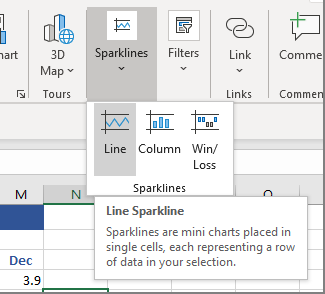
\includegraphics[width=\maxwidth{.65\linewidth}]{gfx/ch08_fig01}
	\caption{The Sparklines Button}
	\label{08:fig01}
\end{figure}

\begin{enumerate}[resume]
		
	\item For the Data Range, enter \fmtTyping{B4:M4}.
	\item For the Location Range, enter \fmtTyping{\$N\$4}.
	\item Click \fmtButton{OK}.
\end{enumerate}

\begin{figure}[H]
	\centering
	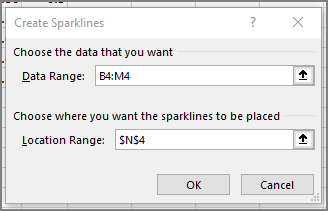
\includegraphics[width=\maxwidth{.65\linewidth}]{gfx/ch08_fig02}
	\caption{The Sparklines Diaglog Box}
	\label{08:fig02}
\end{figure}

Excel creates a tiny line graph that shows the monthly precipitation for the entire year. 

\begin{figure}[H]
	\centering
	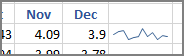
\includegraphics[width=\maxwidth{.50\linewidth}]{gfx/ch08_fig03}
	\caption{One Sparkline}
	\label{08:fig03}
\end{figure}

\begin{enumerate}[resume]
	\item Copy/paste cell \fmtLoc{N4} to \fmtLoc{N5:N13}. The fill handle will make this easier. 
\end{enumerate}

\begin{figure}[H]
	\centering
	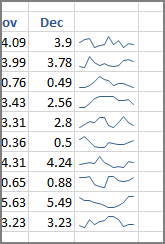
\includegraphics[width=\maxwidth{.50\linewidth}]{gfx/ch08_fig04}
	\caption{All Sparklines In Place}
	\label{08:fig04}
\end{figure}

Now Excel displays a sparkline for each of the cities. While it is not possible to see the details for any specific month and city, it is easy to spot trends. For example, Portland OR has less precipitation in the late summer while Chicago IL seems to start out slow in January and then grow through the spring and early summer. A business manager could use a sparkline to easily detect trends in data.

\begin{enumerate}[resume]
	\item Select \fmtLoc{N4:N13} and notice the \textit{Sparkline Design} tab includes several options to modify the appearance of the sparkline. 
	\item Click \fmtButton{Sparkline Design $ \Rightarrow $ Type $ \Rightarrow $ Column}.
\end{enumerate}

\begin{figure}[H]
	\centering
	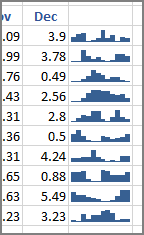
\includegraphics[width=\maxwidth{.50\linewidth}]{gfx/ch08_fig05}
	\caption{Column Sparklines}
	\label{08:fig05}
\end{figure}

The sparklines change into column graphs. The information does not change, but it may be easier to spot trends with one type of graph or the other, so it is a best practice to try both.

\begin{enumerate}[resume]
	\item Open the \fmtWorksheet{Temperature} worksheet in the \fmtWorksheet{CH8-Sparkline} workbook. This worksheet contains the average low temperature for five Alaskan cities\footnote{The climate data is from  \url{https://www.usclimatedata.com/climate/united-states/us}}.
	\item Click cell \fmtLoc{N4} to activate that location.
	\item Click \fmtButton{Insert $ \Rightarrow $ Sparklines $ \Rightarrow $ Win/Loss}.
	\item For the Data Range, enter \fmtTyping{B4:M4}.
	\item For the Location Range, enter \fmtTyping{\$N\$4}.
	\item Click \fmtButton{OK}.
	\item Copy \fmtLoc{N4} to \fmtLoc{N5:N8}.
\end{enumerate}

\begin{figure}[H]
	\centering
	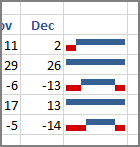
\includegraphics[width=\maxwidth{.50\linewidth}]{gfx/ch08_fig06}
	\caption{Win/Loss Sparkline}
	\label{08:fig06}
\end{figure}

Excel creates a bar graph that shows positive values in blue and negative values in red. This does not show the magnitude of each value, but only whether it is positive or negative in nature. This type of sparkline is useful for quickly determining things like if a stock price is increasing or decreasing.

\begin{enumerate}[resume]
	\item Save and close the \fmtWorksheet{CH8-Sparkline} workbook.
\end{enumerate}

\subsection{Trend Lines}

Excel can easily create trend lines on graphs to indicate data trends. These lines can optionally be extended to forecast how the data may move in the near future.

\begin{enumerate}
	\item Open workbook \fmtWorksheet{CH8-Dow Data}. This workbook contains the closing Dow Jones average for each month from $ 1981 $–$ 1990 $.
	\item Save the workbook as \fmtWorksheet{CH8-Dow}.
	\item Click cell \fmtLoc{A1} to activate that location.
	\item Click \fmtButton{Insert $ \Rightarrow $ Charts $ \Rightarrow $ Recommended Charts}.
	\item Select the line chart (it is the second selection).
	\item Click \fmtButton{OK}.
	\item Click in the chart area to activate it.
	\item Click \fmtButton{Chart Design $ \Rightarrow $ Chart Layouts $ \Rightarrow $ Add Chart Element $ \Rightarrow $ Trendline $ \Rightarrow $ Exponential}. Note: it is reasonable to click on each of the types of trendlines to see which seems to fit the data best.

	\begin{figure}[H]
		\centering
		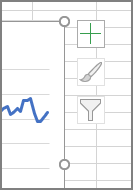
\includegraphics[width=\maxwidth{.50\linewidth}]{gfx/ch08_fig07}
		\caption{Adding A Trendline}
		\label{08:fig07}
	\end{figure}

	\item Excel draws a dotted trendline that shows the growth of the Dow over the ten-year period.

	\begin{figure}[H]
		\centering
		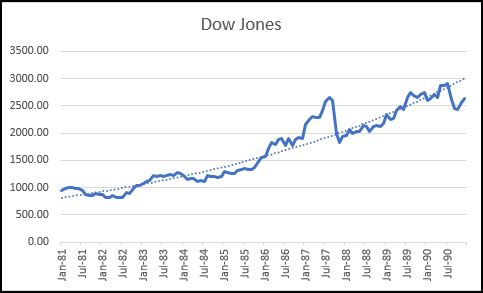
\includegraphics[width=\maxwidth{.95\linewidth}]{gfx/ch08_fig08}
		\caption{Trendline Added to Graph}
		\label{08:fig08}
	\end{figure}

	\item Double-click the dotted trendline to activate it and open the \textit{Format Trendline} properties panel.
	\item Enter \fmtTyping{10} for the \textit{Forward Forcast} period to extend the trendline out five years (ten six-month periods).

	\begin{figure}[H]
		\centering
		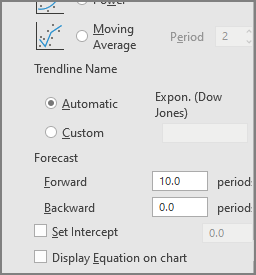
\includegraphics[width=\maxwidth{.50\linewidth}]{gfx/ch08_fig09}
		\caption{Extending The Trendline for 10 Periods}
		\label{08:fig09}
	\end{figure}

	\item Excel forecasts a generally upward trend for the five-year period.

	\begin{figure}[H]
		\centering
		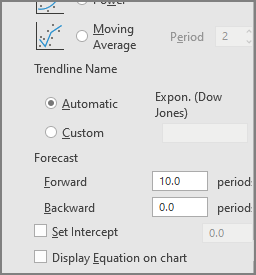
\includegraphics[width=\maxwidth{.95\linewidth}]{gfx/ch08_fig10}
		\caption{Trendline With Forecast}
		\label{08:fig10}
	\end{figure}

\end{enumerate}

\subsection{Forecast Worksheet}

The trend lines described above are easy to add to a chart, but Excel includes a tool called \textit{Forecast Worksheet} that creates a forecast along with confidence levels.

\begin{enumerate}
	\item Click cell \fmtLoc{A1} to activate that location.
	\item Click \fmtButton{Data $ \Rightarrow $ Forecasts $ \Rightarrow $ Forecast Sheet}.
\end{enumerate}

\begin{figure}[H]
	\centering
	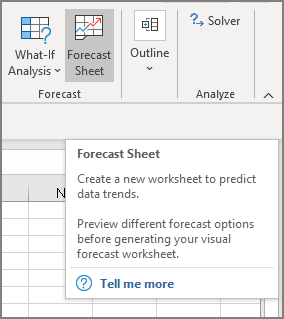
\includegraphics[width=\maxwidth{.65\linewidth}]{gfx/ch08_fig11}
	\caption{The Forecast Sheet Button}
	\label{08:fig11}
\end{figure}

\begin{enumerate}[resume]
	
	\item The \textit{Create Forecast Worksheet} wizard opens with a preview of the worksheet (see Figure \ref{08:fig13}). There are numerous options available but the default options are appropriate for this exercise. Here are what the other options do.
	
	\begin{itemize}
		\item \textbf{Forecast End}. Set an end date for the forecast, which are the orange lines in the illustration.
		\item \textbf{Forecast Start}. Set the start date for the forecast.
		\item \textbf{Confidence interval}. This is a statistical value that indicates a $ 95 $\% certainty that as time progresses the graph will fall between the upper and lower limits shown. The confidence interval can be adjusted, but $ 95 $\% is common.
		\item \textbf{Seasonality}. Excel will search for any sort of seasonal cycles and adjust the forecast accordingly.
		\item \textbf{Timeline and Values Range}. This is the data that was used to create the graph. If Excel got the wrong data ranges then they can be adjusted here.
		\item \textbf{Fill Missing Points Using}. This tells Excel how to deal with data points that are missing. It will either fill those missing values with zero or interpolate a value between the two neighboring values. Interpolation is usually the best option.
		\item \textbf{Aggregate Duplicates Using}. There are a number of options available for aggregating duplicates in the data but \textit{Average} is usually the best option.
	\end{itemize}	
	
	\item Click \fmtButton{Create}.

\end{enumerate}

\begin{figure}[H]
	\centering
	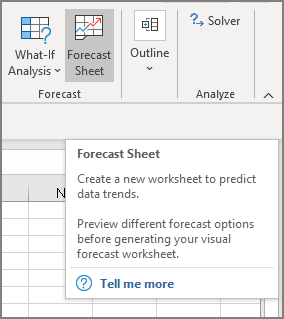
\includegraphics[width=\maxwidth{.95\linewidth}]{gfx/ch08_fig12}
	\caption{Dow Forecast}
	\label{08:fig12}
\end{figure}

\begin{enumerate}[resume]
	\item Excel creates a new worksheet containing the chart along with a table listing all of the values used to create the chart.
	\item Rename \fmtWorksheet{Sheet1} to \fmtTyping{Forecast}.
	\item Scroll to the bottom of the table to see the values Excel forecast to extend the graph. Those values can be used to forecast the Dow Jones for a specific date; so the Dow was forecast to be at $ 2389.37 $ in January $ 1991 $.
	\item Save and close the \fmtWorksheet{CH8-Dow} workbook.
\end{enumerate}

Following is a second example of a forecast worksheet that uses beer production data because it shows a clear seasonal trend over time.

\begin{enumerate}
	\item Open workbook \fmtWorksheet{CH8-Beer Data}. This workbook contains the total monthly United States beer production, in barrels, for January, $ 1980 $, until December, $ 1991 $. 
	\item Save the workbook as \fmtWorksheet{CH8-Beer}.
	\item Click in \fmtLoc{A1} to select that location.
	\item Click \fmtButton{Data $ \Rightarrow $ Forecast $ \Rightarrow $ Forecast Sheet}.
	\item Accept the default options and click \fmtButton{Create}.
	\item The graph clearly shows the cyclic nature of beer production and forecasts a similar cycle out to December, $ 1994 $.
	\item Rename \fmtWorksheet{Sheet1} to \fmtTyping{Forecast}.
	\item After viewing the forecast sheet, save and close the \fmtWorksheet{CH8-Beer} workbook.
\end{enumerate}

\begin{figure}[H]
	\centering
	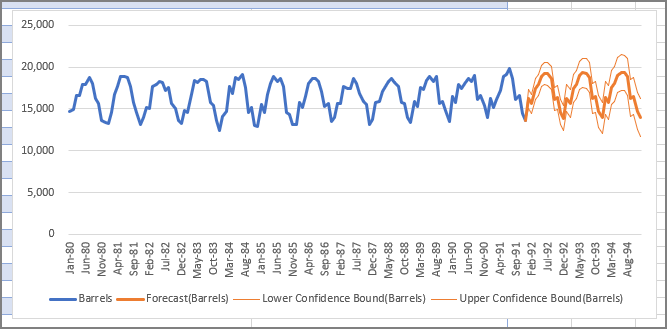
\includegraphics[width=\maxwidth{.95\linewidth}]{gfx/ch08_fig13}
	\caption{Beer Production Forecast}
	\label{08:fig13}
\end{figure}

A forecast sheet is a simple method business owners use to predict business cycles like customer demand so owners can manage inventory, hire help, or take other actions.

\subsection{3D Maps}

Excel includes a feature called \textit{$ 3 $D Maps} that merge geographically-oriented maps with a time line so business owners can look for trends over time in various geographical areas they service. As an example, if a company markets to an entire state then the owner can create a \textit{$ 3 $D Map} that shows sales by county over the preceding five years, and that may make important trends obvious.

\textit{$ 3 $D Maps} combines map and time line data in a feature called \textit{Tours}. The process can be somewhat intimidating at first, but becomes easier with practice.

\subsubsection{Arizona Population Growth}

\begin{enumerate}
	\item Open workbook \fmtWorksheet{CH8-Map Data}. This workbook contains two worksheets.
	
	\begin{itemize}
		\item \textbf{AZ Population}. This worksheet lists the population for all Arizona counties from $ 1969 $ until $ 2018 $, by year.\footnote{This data was found at the United States Bureau of Economic Analysis, \url{https://apps.bea.gov/iTable/iTable.cfm?reqid=70&step=1&isuri=1&acrdn=7\#reqid=70&step=1&isuri=1&acrdn=7}} Note: La Paz County was separated from Yuma County on January $ 1 $, $ 1983 $ so the Yuma data contains counts of people who lived in what became La Paz County through $ 1982 $ and excludes it beginning with $ 1983 $.
		\item \textbf{GDP}. This worksheet contains the real \textit{Gross Domestic Product} (in millions of dollars) for each of the fifty states, and Washington D.C., from $ 2010 $ until $ 2015 $, by economic sector.\footnote{The GDP information was found at \url{http://proximityone.com/gdpbyindustry.htm}.} The table also includes a \textit{Quantity Index} for each year which indicates the percent change in each value when compared to the base year, $ 2009 $.
	\end{itemize}
	
	\item Save the workbook as \fmtWorksheet{CH8-Maps}.
	\item In the \fmtWorksheet{AZ Population} worksheet, click cell \fmtLoc{A1} to activate that location.
	\item Click \fmtButton{Insert $ \Rightarrow $ Tours $ \Rightarrow $ $ 3 $D Map}.
\end{enumerate}

\begin{center}
	\begin{infobox}{Information}
		\textbf{Enable $ 3 $D Maps}
		\\
		\\
		The first time \textit{$ 3 $D Maps} is started, Excel pops up the warning illustrated in Figure \ref{08:fig20}. The module only needs to be enabled one time, so click \fmtButton{Enable}.

		\begin{figure}[H]
			\centering
			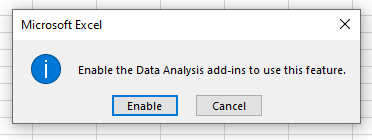
\includegraphics[width=\maxwidth{.85\linewidth}]{gfx/ch08_fig20}
			\caption{Enable $ 3 $D Maps}
			\label{08:fig20}
		\end{figure}

	\end{infobox}
\end{center}

\begin{enumerate}[resume]
	\item The \textit{$ 3 $D Maps} editor box, Figure \ref{08:fig21}, looks complex. Here is an explanation of each of the four main areas.

	\begin{figure}[H]
		\centering
		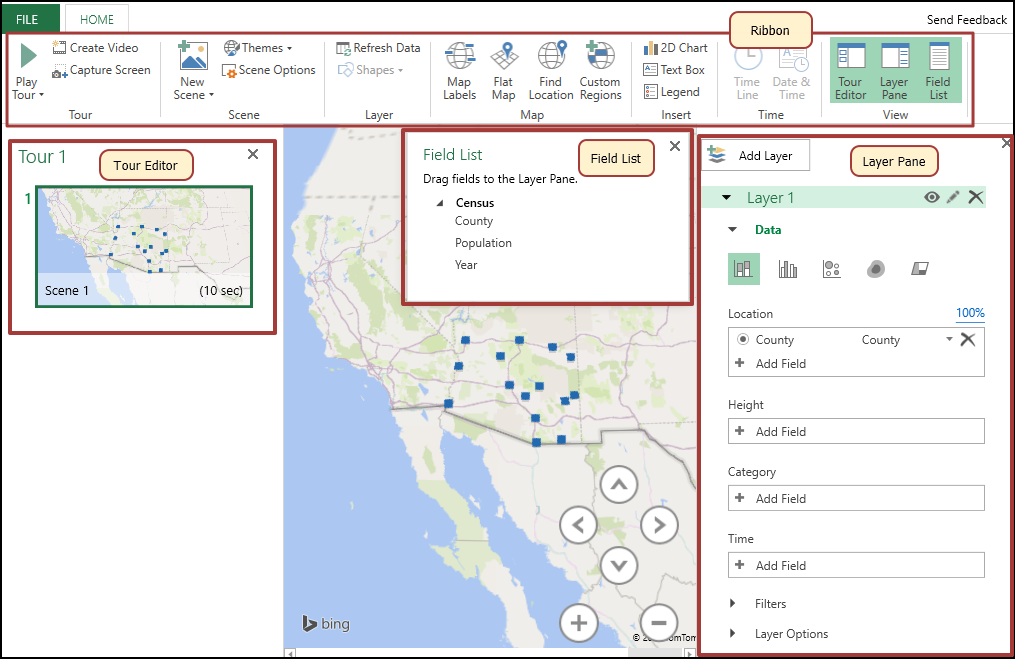
\includegraphics[width=\maxwidth{.95\linewidth}]{gfx/ch08_fig21}
		\caption{$ 3 $D Map Editor}
		\label{08:fig21}
	\end{figure}
	
	\begin{itemize}
		\item \textbf{Ribbon}. The \textit{$ 3 $D Map} ribbon (Figure \ref{08:fig22}) serves the same function as in any Microsoft program. It contains buttons to activate the most commonly-used mapping functions. The various buttons will be used throughout this lesson and their functions will become clear through use.

		\begin{figure}[H]
			\centering
			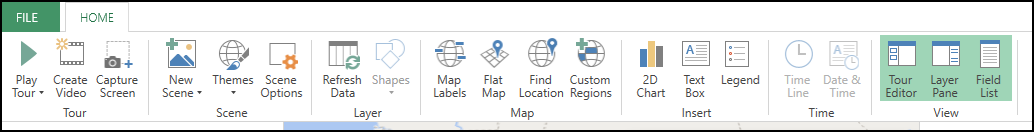
\includegraphics[width=\maxwidth{.95\linewidth}]{gfx/ch08_fig22}
			\caption{$ 3 $D Map Ribbon}
			\label{08:fig22}
		\end{figure}

		\item \textbf{Tour Editor}. Each \textit{$ 3 $D Map} is divided into scenes that are contained in a \textit{Tour}. The \textit{Tour Editor}, on the left side of the screen, (Figure \ref{08:fig23}) is where settings like the length of time for each scene is defined.

		\begin{figure}[H]
			\centering
			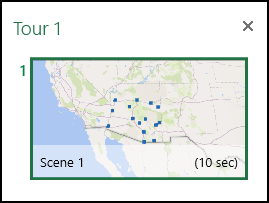
\includegraphics[width=\maxwidth{.50\linewidth}]{gfx/ch08_fig23}
			\caption{$ 3 $D Map Tour Editor}
			\label{08:fig23}
		\end{figure}

		\item \textbf{Field List}. The various fields (columns) in the original dataset are listed here (Figure \ref{08:fig24}) so they can be used on the map. This is a pop-up dialog box and can be moved as desired.

		\begin{figure}[H]
			\centering
			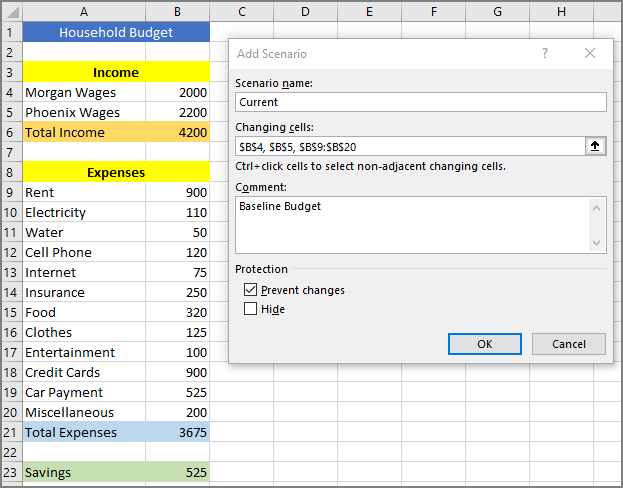
\includegraphics[width=\maxwidth{.50\linewidth}]{gfx/ch08_fig24}
			\caption{$ 3 $D Map Field List}
			\label{08:fig24}
		\end{figure}

		\item \textbf{Layer Pane}. $ 3 $D Maps are composed of multiple layers and this pane is where settings for each of the layers are specified.

		\begin{figure}[H]
			\centering
			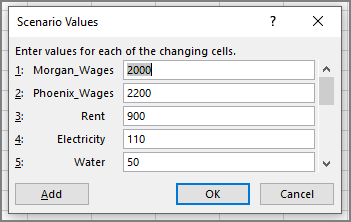
\includegraphics[width=\maxwidth{.65\linewidth}]{gfx/ch08_fig25}
			\caption{$ 3 $D Map Layer Pane}
			\label{08:fig25}
		\end{figure}

	\end{itemize}
	
\end{enumerate}


\begin{enumerate}[resume]
	\item The \textit{Layers Pane} is where most of the work is done for a \textit{$ 3 $D Map}. It is divided into three main sections.
	
	\begin{itemize}
		\item \textbf{Data}. This section is where the data used in the map is manipulated. Figure \ref{08:fig26} illustrates the settings found in the data section.

		\begin{itemize}
			\item \textbf{Type of Visualization}. At the top of the pane are five buttons that change the map display setting to a stacked column, clustered column, bubble, heat map, and region. Changing the visualization is as easy as clicking one of the buttons, so they should all be applied to see which gives the best representation of the data.
			\item \textbf{Location}. This setting divides the map into geographical locations. Maps can use data for country, state, county, city, and many other regional types. For example, a sales map may show sales by state or sales by city.
			\item \textbf{Height}. This setting determines the height of the data column on a graph. The data needs to be numeric so it can be converted into a column height.
			\item \textbf{Category}. This setting contains categories for the values graphed by height. For example, a sales map may include categories for electronics, clothing, or other merchandise.
			\item \textbf{Time}. This setting contains the time value being graphed. \textit{$ 3 $D Maps} can be created to display a period of time, like the value of monthly or weekly sales, but maps can also be created that do not have a time component.
		\end{itemize}		

		\item \textbf{Filters}. This section permits the creation and application of complex filters for the data being charted.
		\item \textbf{Layer Options}. This section is where various options, like color, are set for the displayed data.
	\end{itemize}

	\begin{figure}[H]
		\centering
		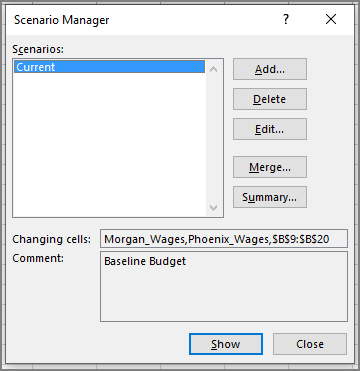
\includegraphics[width=\maxwidth{.60\linewidth}]{gfx/ch08_fig26}
		\caption{Layers Pane}
		\label{08:fig26}
	\end{figure}

	\item By default, Excel detects the data field that contains geographical information and automatically adds that field to the \fmtButton{Location} setting. For \textit{AZ Population}, county names are the geographical information and that field is added to the \textit{Location} setting. As soon as the county names are added, a stacked column is placed in each county on the map. Since there is no \textit{Height} data available yet, those columns are only flat squares on the map.
	\item Click and drag \textit{Population} in the \textit{Field List} to the \fmtButton{Height} setting. Excel immediately applies the sum of the population values to the counties and the columns react accordingly (see Figure \ref{08:fig27}). Notice the middle column, for Maricopa county, is quite long while the other counties are shorter. Also, Excel creates a legend box to show that the blue columns are the population.

	\begin{figure}[H]
		\centering
		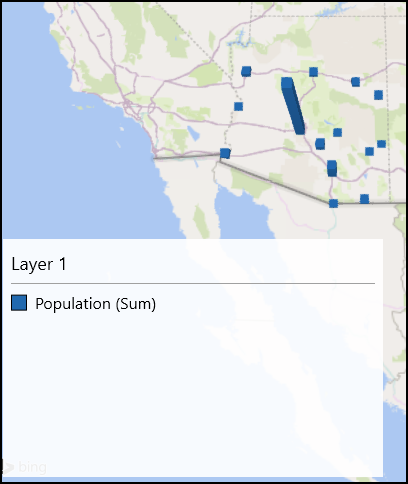
\includegraphics[width=\maxwidth{.75\linewidth}]{gfx/ch08_fig27}
		\caption{Population Added to Height}
		\label{08:fig27}
	\end{figure}

	\item By default, \textit{Population} will display the sum of population over time. For example, if Cochise County had $ 40,000 $ people one year and $ 50,000 $ the next, Excel will display $ 90,000 $ as the county population. Instead of summing the population over the years, it is more appropriate to display only the current year. Click the drop-down arrow for \textit{Population}, select \fmtButton{No Aggregation}. After changing the aggregation, the columns change to an orange color.
	\item Click the triangle beside \fmtButton{Layer Options} to open that setting.
	\item Set the Thickness for the column to $ 200\% $.
	\item Click the color drop-down for \textit{Population (No Aggregation)} and choose blue.

	\item Click and drag \textit{Year} in the \textit{Field List} to the \fmtButton{Time} setting. Not much changes, but a time line bar is added to the bottom of the map. The small triangle marker under the time line can be moved left and right to display the population for any desired point of time.
	\item Click the down arrow to the right of \textit{Year} in the \textit{Time} setting and select \fmtButton{Year} in the drop down list.
	\item Click \fmtButton{Play Tour} at the left edge of the ribbon. Excel will ``play'' the entire timeline in ten seconds (that timing can be changed). When the video is finished playing, click the left-arrow button in the lower left corner of the video screen to return to the map editor.
	\item Click the \fmtButton{Pencil} icon to edit \textit{Layer 1} in the \textit{Layers Pane} and change the name of the layer to \fmtTyping{Population}.

	\item Click \fmtButton{Add Layer} at the top of the \textit{Layer Pane}. Excel adds a new layer under the \textit{Population} layer.
	\item Rename \textit{Layer 2} to \fmtTyping{Counties}.
	\item By default, Excel places the \textit{County} data field in \textit{Location}. Leave this in place.
	\item Click and drag \textit{County} from the \textit{Field List} to \textit{Category}. The \textit{County} data field is now in two settings, \textit{Location} and \textit{Category}. Excel now treats each county as a separate category and colors the columns different colors for each county.
	\item Click \fmtButton{Region} on the visualization bar (it is the last option). The \textit{Region} button is outlined in red in Figure \ref{08:fig28}. The counties are now colored so they are easy to see. 
\end{enumerate}

\begin{figure}[H]
	\centering
	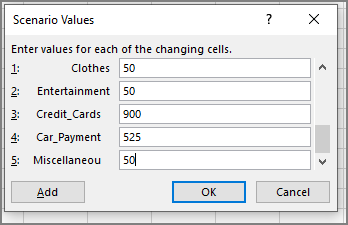
\includegraphics[width=\maxwidth{.85\linewidth}]{gfx/ch08_fig28}
	\caption{County Areas Colored}
	\label{08:fig28}
\end{figure}

\begin{enumerate}[resume]
	\item The county colors are a bit bright, so click the triangle beside \fmtButton{Layer Options} to open that setting.
	\item Move the \textit{Opacity} slider to about $ 50\% $. That will dim the county colors while leaving the population columns the same.
	\item Notice that each county's color can be set using the color dropdown, so it would be easy to highlight a county in some bright color like red while using duller colors for the other counties.
	\item Click the \fmtButton{Play Tour} button to see what the tour looks like with the county colors.
	\item Click the \textit{Population} layer to activate it again.
	\item Click through each of the five types of visualizations and play the tour using each visualization to see which type works best for this data. For this tutorial, leave the visualization on \textit{Heat Map}.
\end{enumerate}

At this point, this tour is nearly done. However, there are just a few settings that can be tweaked a bit.

\begin{enumerate}[resume]
	\item Click \textit{Tour 1} at the top of the \textit{Tour Editor} and enter \fmtTyping{Population}. 
	\item Excel's \textit{$ 3 $D Map} is drawn on a globe so data for countries around the world can be displayed. It is better for this map to be displayed flat rather than on a globe. Click \fmtButton{Flat Map} in the ribbon to convert the map from a globe to a flat map. The map can always be reverted to a globe if desired.
	\item Having the time displayed on the tour is distracting, so format the displayed date to only show the year. Right-click the date displayed on the screen and select \fmtButton{Edit}. In the edit box, choose the \textit{Time Format} that only shows the year without the month and day, then click \fmtButton{Accept}.
	\item The legend is not needed for this map, so click that box and delete it. Note: both layers create a legend and both should be deleted. Either legend can be turned back on if desired by clicking the \fmtButton{Legend} button on the ribbon.
	\item Click and drag the map to center Arizona in the display. Also, experiment with the four arrow and plus/minus buttons to adjust the display.
	\item Click the \fmtButton{Scene Options} button on the ribbon. Change the name of the scene to \fmtTyping{Population}. The defaults for the other options are appropriate for this tour, but could be adjusted for other tours.
	\item Close the \textit{Scene Options} dialog box.
	\item Click \fmtButton{Themes} to explore the themes available for tours. The first theme, which is default, is appropriate for this tour, but it is easy to apply other themes.
	\item Click \fmtButton{Map Labels} to turn on the labels. While only the largest cities are named, the labels help to identify Phoenix and Tucson.
	\item Click \fmtButton{Tour Editor}, \fmtButton{Layer Pane}, and \fmtButton{Field List }to turn off those dialog boxes. These can always be turned back on if desired.
	\item Figure \ref{08:fig29} illustrates the final Population Map.
\end{enumerate}

\begin{figure}[H]
	\centering
	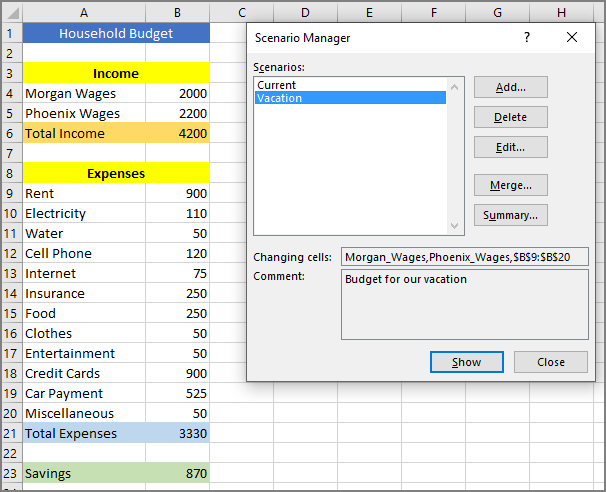
\includegraphics[width=\maxwidth{.50\linewidth}]{gfx/ch08_fig29}
	\caption{Final Population Map}
	\label{08:fig29}
\end{figure}

There are only two other buttons on the ribbon that have not been described.

\begin{enumerate}[resume]
	\item \textbf{Create Video}. This will create a video of the tour that would be suitable to play online (YouTube) or on a desktop.
	\item \textbf{Capture Screen}. This button copies the screen to the clipboard so it can later be pasted in a PowerPoint slide or other report.
	\item To save the map, click \fmtButton{File $ \Rightarrow $ Close}. The map is saved as part of the workbook and will be available the next time the workbook is opened. 
\end{enumerate}

Excel also adds a text box to the active worksheet to let users know that there are \textit{$ 3 $D Map} tours available in the workbook (see Figure \ref{08:fig30}).

\begin{figure}[H]
	\centering
	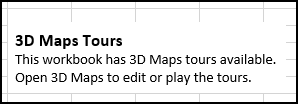
\includegraphics[width=\maxwidth{.65\linewidth}]{gfx/ch08_fig30}
	\caption{$ 3 $D Maps Are Available}
	\label{08:fig30}
\end{figure}

\subsubsection{Gross Domestic Product}

As a second example of a \textit{$ 3 $D Map}, the states' \textit{Gross Domestic Product} (GDP) for several different sectors will be mapped.

\begin{enumerate}
	\item Open the \fmtWorksheet{GDP} worksheet in \fmtWorksheet{CH8-Maps}.
	\item Click in \fmtLoc{A1} to activate that cell.
	\item Click \fmtButton{Insert $ \Rightarrow $ Tours $ \Rightarrow $ $ 3 $D Map}.
	\item The \textit{Population} tour is listed and could be edited, but click \fmtButton{New Tour} to map the GDP data.
	\item If necessary, activate the \textit{Tour Editor}, \textit{Layer Pane}, and \textit{Field List} by clicking those buttons in the ribbon.
	\item If Excel did not automatically place the \textit{State} data field in the \fmtButton{Location} setting, then click and drag \textit{State} in the \textit{GDP Field List} to the \fmtButton{Location} setting. 
	\item Click the down arrow to the right of \textit{State} in the \fmtButton{Location} setting and select \fmtButton{State/Province} in the drop down list.
	\item Click and drag \textit{GDP2015} in the \textit{GDP Field List} to the \fmtButton{Height} setting.
	\item Click the down-arrow to the right of \textit{GDP2015 (Sum)} and select \fmtButton{Maximum}.
	\item Click and drag \textit{Sector} in the \textit{GDP Field List} to the \fmtButton{Category} setting.
	\item Click the pencil icon beside \textit{Layer 1} and change the name of this layer to \fmtTyping{GDP 2015}.
	\item Change the visualization type to \fmtButton{Clustered Column} (the second selection).
	\item Excel displays all $ 15 $ sectors for each state, but that is too many to be useful. Click the triangle arrow beside \fmtButton{Filters} to open that setting then click \fmtButton{Add Filter}.
	\item Select \fmtButton{Sector} from the filters list.
	\item In the \textit{Sector} filter, check \fmtButton{Agriculture, forestry, fishing, and hunting}; \fmtButton{Construction}; \fmtButton{Manufacturing}; and \fmtButton{Mining}.
	\item Click \fmtButton{Flat Map} and then adjust the map to fit on the screen. Remember that Alaska and Hawaii need to be visible on the map. Also, experiment with the four arrow and plus/minus buttons to adjust the display in order to get the best view of the columns.
	\item Move and resize the legend so it displays all four sectors without a lot of wasted space and also it does not cover Hawaii.
	\item The colors used for the four sectors are difficult to differentiate. Click the triangle arrow beside \fmtButton{Layer Options} to open that setting. In the \textit{Color} section, select each of the sectors and choose a color that makes it easy to differentiate from other sectors.
	\item Also in the \textit{Layer Options}, adjust the thickness of the columns to about $ 200\% $.
	\item Click \textit{Tour 1} at the top of the \textit{Tour Editor}. Enter \fmtTyping{GDP} as the name of the tour. 
	\item Click the \fmtButton{Scene Options} button on the ribbon. Change the name of the scene to \fmtTyping{Industry}. In the Effects section, select a transition of $ 3 $ seconds, \textit{Fly Over} as the effect, and adjust the \textit{Effect Distance} slider to about $ 75\% $ to the right.
	\item Close the \textit{Scene Options} dialog box.
	\item Click \fmtButton{Text Box} to add a text box to the tour. For \textit{Title}, enter \fmtTyping{Industry}. For Description, enter \fmtTyping{GDP for four industrial sectors: Agriculture, Construction, Manufacturing, and Mining.} Select white as the background color for the text box.
	\item Click \fmtButton{Create} to create the text box and close the dialog.
	\item Position and resize the text box over Canada so it does not cover data displayed for the United States.
	\item Click \fmtButton{Map Labels} to turn on the labels.
	\item Figure \ref{08:fig31} illustrates the final Industry Map.
	
	\begin{figure}[H]
		\centering
		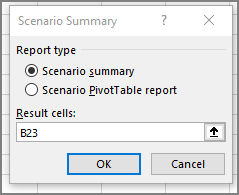
\includegraphics[width=\maxwidth{.95\linewidth}]{gfx/ch08_fig31}
		\caption{Industry $ 3 $D Map}
		\label{08:fig31}
	\end{figure}
	
	\item Play the tour to see what it looks like. The map size and orientation (using the arrow buttons on the map), along with the locations for the legend and text box can be adjusted for the best possible display.
	
	\item Add a second scene for this tour. Click the \fmtButton{New Scene} drow-down arrow and select \fmtButton{Copy Industry}. Excel will create a copy of the \textit{Industry} scene so only a few changes need to be made to continue the tour.
	\item Click the \fmtButton{Scene Options} button on the ribbon. Change the name of the scene to \fmtTyping{Service} and the \textit{Effect} to \fmtButton{Circle}. Close the \textit{Scene Options} dialog.
	\item While the \textit{Service} scene is active, open the \fmtButton{Filters} setting and uncheck everything, then check \fmtButton{Education services, health care, and social assistance}; \fmtButton{Finance, insurance, real estate, rental, and leasing}; \fmtButton{Information}; and \fmtButton{Other services, except government}.
	\item Click the triangle arrow beside \fmtButton{Layer Options} to open that setting. In the \textit{Color} section, select each of the sectors and choose a color that makes it easy to differentiate from other sectors.
	\item Double-click the text box and change the title to \fmtTyping{Service} and the description to \fmtTyping{GDP for four service sectors: Education, Finance, Information, and Other}.
	
	\item Add a final scene for this tour. Click the \fmtButton{New Scene} drop-down arrow and select \fmtButton{Copy Service}. Excel will create a copy of the \textit{Service} scene so only a few changes need to be made to continue the tour.
	\item Click the \fmtButton{Scene Options} button on the ribbon. Change the name of the scene to \fmtTyping{Retail} and the \textit{Effect} to \fmtButton{Push In}. Close the \textit{Scene Options} dialog box.
	\item While the \textit{Retail} scene is active, open the \fmtButton{Filters} setting and uncheck everything, then check \fmtButton{Professional and business services}; \fmtButton{Retail trade}; and \fmtButton{Transportation and warehousing}.
	\item Click the triangle arrow beside \fmtButton{Layer Options} to open that setting. In the \textit{Color} section, select each of the sectors and choose a color that makes it easy to differentiate from other sectors.
	\item Double-click the text box and change the title to \fmtTyping{Retail} and the description to \fmtTyping{GDP for three retail sectors: Professional Services, Retail Trade, and Transportation and Warehousing.}
	
	\item Click \fmtButton{Tour Editor}, \fmtButton{Layer Pane}, and \fmtButton{Field List} to turn off those dialog boxes. These can always be turned back on if desired.
	\item Play the tour to see the completed \textit{$ 3 $D Maps Tour}.
	\item To save the map, click \fmtButton{File $ \Rightarrow $ Close}. The map is saved as part of the workbook and will be available the next time the workbook is opened.
	\item Save and close the \fmtWorksheet{CH8-Maps} workbook.
	
\end{enumerate}

The two maps created in this lesson are simple but demonstrate the two most powerful \textit{$ 3 $D Maps} concepts: $ 1 $) Using a time line to focus on a change in data over a defined term, and $ 2 $) building a tour by combining two or more scenes. Excel's \textit{$ 3 $D Map} is a powerful decision-support tool and any time spent mastering it is worthwhile.

\begin{center}
	\begin{tkwbox}{Key Take-Aways}
		\textbf{Advanced Charts}
		\\
		\begin{itemize}
			\setlength{\itemsep}{0pt}
			\setlength{\parskip}{0pt}
			\setlength{\parsep}{0pt}
			
			\item Sparklines graphically represent data trends in a single cell. These are quick and easy to add to a worksheet and provide managers readily available important information.
			\item Trend lines simplify graphs by displaying a single trend line to summarize the general direction of the data. There are several different trend lines available in Excel and those lines can be modified to enhance their appearance.
			\item Forecast Worksheets create a trend line that includes confidence levels. These worksheets are also more robust than simple trend lines and can analyze cyclic or seasonal data.
			\item $ 3 $D Maps are powerful visual representations of both geographic and time dimensions to enhance decision-making.
			
		\end{itemize}
	\end{tkwbox}
\end{center}

\section{What-If Analysis}

\begin{center}
	\begin{objbox}{Learning Objectives}
		\begin{itemize}
			\setlength{\itemsep}{0pt}
			\setlength{\parskip}{0pt}
			\setlength{\parsep}{0pt}
			
			\item Data tables permit numeric analysis of the result of changing inputs.
			\item Scenarios create various sets of inputs to compare the resulting output.
			\item Goal seeking finds an optimum input to achieve a specific goal.
			\item The Solver performs complex analysis of a scenario and adjusts various parameters for an optimum outcome.
			
		\end{itemize}
	\end{objbox}
\end{center}

\subsection{Data Tables}

Data tables display a range of results for a formula or function as one or two input variables are automatically cycled through a list. Managers can quickly compare potential options to determine a course of action.

\subsubsection{One-Variable Data Table}

As an example of a one-variable data table, imagine that the owner of a small theater wants to predict revenue for the upcoming season. If the revenue from a single ticket sale can be calculated, then that can be put into a formula so revenue projections can be derived.

\begin{enumerate}
	\item Open a new blank workbook.
	\item Save the workbook as \fmtWorksheet{CH8-Data Table}.
	\item Rename \fmtWorksheet{Sheet1} to \fmtTyping{Revenue}.
	\item Enter the following labels (see Figure \ref{08:fig40}).
	
	\begin{itemize}
		\item In cell \fmtLoc{A1} enter \fmtTyping{Ticket Sales Last Season}.
		\item In cell \fmtLoc{A2} enter \fmtTyping{Revenue Per Ticket}.
		\item In cell \fmtLoc{A3} enter \fmtTyping{Revenue Last Season}.
		\item In cell \fmtLoc{A4} enter \fmtTyping{Projected Growth}.
		\item In cell \fmtLoc{A5} enter \fmtTyping{Revenue This Season}.
	\end{itemize}
	
	\item Adjust the width of \fmtLoc{Column A} so the labels fit in the column.
	\item Name cells \fmtLoc{B1:B5}. Do this by right-clicking each cell and select \fmtButton{Define Name} from the drop-down menu. Use the default names Excel suggests.

	\begin{itemize}
		\item Cell \fmtLoc{B1}: \fmtTyping{Ticket\_Sales\_Last\_Season}
		\item Cell \fmtLoc{B2}: \fmtTyping{Revenue\_Per\_Ticket}
		\item Cell \fmtLoc{B3}: \fmtTyping{Revenue\_Last\_Season}
		\item Cell \fmtLoc{B4}: \fmtTyping{Growth}
		\item Cell \fmtLoc{B5}: \fmtTyping{Revenue\_This\_Season}
	\end{itemize}

	\item Enter the following values in \fmtLoc{Column B}.

	\begin{itemize}
		\item In cell \fmtLoc{B1} enter \fmtTyping{20000}. This is the number of tickets sold last season and will serve as a start point for this season's projection.
		\item In cell \fmtLoc{B2} enter \fmtTyping{8}. This is the average revenue, \$$ 8.00 $, that a single ticket generates.
		\item In cell \fmtLoc{B3} enter \fmtTyping{=Ticket\_Sales\_Last\_Season * Revenue\_Per\_Ticket
		}. This is the total revenue from last season. 
		\item In cell \fmtLoc{B4}, enter \fmtTyping{0}. For this analysis, the first assumption is that there is zero growth in ticket sales over last season. This provides a baseline for the other analysis.
		\item In cell \fmtLoc{B5}, enter \fmtTyping{=Ticket\_Sales\_Last\_Season * Revenue\_Per\_Ticket + (Projected\_Growth * Ticket\_Sales\_Last\_Season)
		}
	\end{itemize}

	\item Format the following cells.

	\begin{itemize}
		\item Cell \fmtLoc{B1}: Comma
		\item Cell \fmtLoc{B2}: Accounting
		\item Cell \fmtLoc{B3}: Comma
		\item Cell \fmtLoc{B4}: Percent
		\item Cell \fmtLoc{B5}: Comma
	\end{itemize}

\end{enumerate}

\begin{figure}[H]
	\centering
	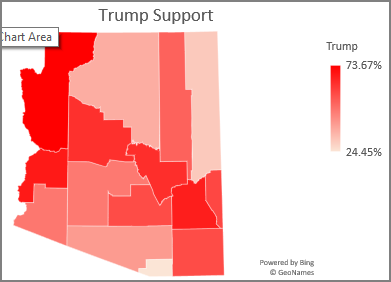
\includegraphics[width=\maxwidth{.65\linewidth}]{gfx/ch08_fig40}
	\caption{The Data Table Parameters}
	\label{08:fig40}
\end{figure}

\begin{enumerate}[resume]
	 
	\item Next, set up the data table area.

\begin{itemize}
	\item In cell \fmtLoc{D2}, enter \fmtTyping{Projection}. Bold that cell.
	\item In cell \fmtLoc{D3}, enter \fmtTyping{Growth}.
	\item In cell \fmtLoc{E3}, enter \fmtTyping{Revenue}.
	\item Leave cell \fmtLoc{D4} blank.
	\item In cells \fmtLoc{D5:D14}, enter \fmtTyping{$ 0.005 $}, \fmtTyping{$ 0.01 $}, \fmtTyping{$ 0.015 $}, \fmtTyping{$ 0.02 $}, \fmtTyping{$ 0.025 $}, \fmtTyping{$ 0.03 $}, \fmtTyping{$ 0.035 $}, \fmtTyping{$ 0.04 $}, \fmtTyping{$ 0.045 $} and \fmtTyping{$ 0.05 $}. \textit{Note}: autofill will help with this task.
	\item Format \fmtLoc{Column D} as percents and increase the decimal places to two. When done, cell \fmtLoc{D5} should read $ 0.50 $\%.
	\item In cell \fmtLoc{E4}, enter \fmtTyping{=Revenue\_This\_Season}. This will ``seed'' the revenue formula used in cell \textit{B5} into the data table.
\end{itemize}

	\item Select \fmtLoc{D4:E14} to contain the data table.
	\item Click \fmtButton{Data $ \Rightarrow $ Forecast $ \Rightarrow $ What-If Analysis $ \Rightarrow $ Data Table}.
	\item Leave the \textit{Row input cell} box empty since this data table only calculates data in a column. In the \textit{Column input cell} box, enter \fmtTyping{Projected\_Growth}, which is the name for cell \textit{B4}, the projected growth rate. Figure \ref{08:fig41} illustrates the completed Data Table dialog box.
	
\end{enumerate}

\begin{figure}[H]
	\centering
	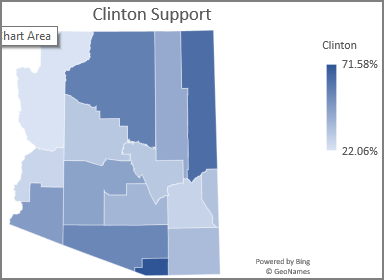
\includegraphics[width=\maxwidth{.95\linewidth}]{gfx/ch08_fig41}
	\caption{Setting Up the Data Table}
	\label{08:fig41}
\end{figure}

\begin{enumerate}[resume]	
	\item Click \fmtButton{OK}.
	\item Format \fmtLoc{Column E} as \textit{Comma} format.
\end{enumerate}

\begin{figure}[H]
	\centering
	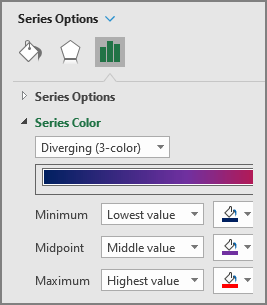
\includegraphics[width=\maxwidth{.95\linewidth}]{gfx/ch08_fig42}
	\caption{One-Variable Data Table}
	\label{08:fig42}
\end{figure}

The data table displays the projected revenue for each of the growth rates in \fmtLoc{Column D}. This analysis assumes that the number of tickets sold will increase. However, it is possible that ticket sales will decrease. Change the values in cells \textit{D5:D14} so some are negative and notice that the projected revenue automatically updates to display losses.

\begin{figure}[H]
	\centering
	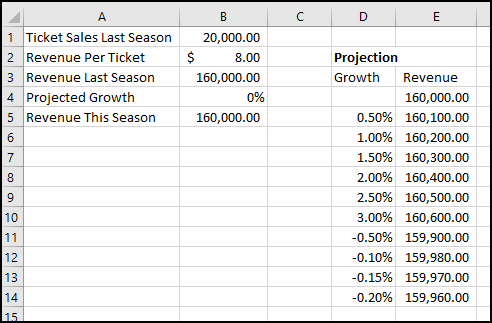
\includegraphics[width=\maxwidth{.95\linewidth}]{gfx/ch08_fig43}
	\caption{One-Variable Data Table With Negative Values}
	\label{08:fig43}
\end{figure}

\begin{enumerate}[resume]
	\item Save the \fmtWorksheet{CH8-Data Table} workbook.
\end{enumerate}

\subsubsection{Two-Variable Data Table}

A mortgage is one of the most common loans. A mortgage for a home is a huge investment and borrowers must think carefully about the size of the monthly payment compared to their disposable income. A two-variable data table is very helpful in this type of decision.\footnote{See Chapter \ref{ch02:computations}, \nameref{ch02:computations}, page \pageref{ch02:computations} for more information about computing loans like mortgages.}

Mortgages are commonly written for $ 10 $ to $ 30 $ year terms and the interest rate can vary widely, depending on many factors. For this example, assume the interest rate is between $ 5\% $ and $ 8.5\% $.

\begin{enumerate}
	\item Open a new worksheet in the \fmtWorksheet{CH8-Data Table} workbook.
	\item Name the worksheet \fmtWorksheet{Mortgage}.
	\item Enter the following labels.
	
	\begin{itemize}
		\item In cell \fmtLoc{A1} enter \fmtTyping{Loan Amount}.
		\item In cell \fmtLoc{A2} enter \fmtTyping{Term in Years}.
		\item In cell \fmtLoc{A3} enter \fmtTyping{Interest Rate}.
		\item In cell \fmtLoc{A4} enter \fmtTyping{Payment}.
	\end{itemize}

	\item Adjust the width of \fmtLoc{Column A} so the labels fit in the column.
	\item To start the data table, enter these values in \fmtLoc{Column B}.
	
	\begin{itemize}
		\item In cell \fmtLoc{B1} enter \fmtTyping{100000}. This is the amount being borrowed.
		\item In cell \fmtLoc{B2} enter \fmtTyping{10}. This is the number of years to pay off the loan.
		\item In cell \fmtLoc{B3} enter \fmtTyping{0.05}. This is the interest rate being charged for the loan. \textit{Note}: the data table may be easier to read if cell \fmtLoc{B3} is formatted as \textit{percent} rather than \textit{general}. If the format is changed, be certain that it reads $ 5\% $.
		\item In cell \fmtLoc{B4}, enter \fmtTyping{=PMT(B3/12,B2*12,B1)}. Given the information in \fmtLoc{B1:B3}, Excel calculates a payment of $ \$1,060.66 $ per month. This is a negative amount since the payment is going out of the borrower's savings.
	\end{itemize}

	\item Next, set up the data table area.
	\item In cell \fmtLoc{D4}, enter \fmtTyping{=B4}. This will ``seed'' the \fmtButton{PMT} formula into the data table.
	\item In cells \fmtLoc{D5:D12}, enter \fmtTyping{0.05}, \fmtTyping{0.055}, \fmtTyping{0.06}, \fmtTyping{0.065}, \fmtTyping{0.07}, \fmtTyping{0.075}, \fmtTyping{0.08}, and \fmtTyping{0.085}.
	\item Format \fmtLoc{D5:D12} as percents with two decimal places.
	\item In cells \fmtLoc{E4:I4}, enter \fmtTyping{10}, \fmtTyping{15}, \fmtTyping{20}, \fmtTyping{25}, and \fmtTyping{30}.
	\item Select \fmtLoc{D4:I12} to contain the data table.
	\item Click \fmtButton{Data $ \Rightarrow $ Forecast $ \Rightarrow $ What-If Analysis $ \Rightarrow $ Data Table}.
	\item In the \textit{Row input cell} box, enter the reference for the data found in \textit{Row 4}. In the example, \textit{Row 4} contains the loan term, and that is found in cell \fmtLoc{\$B\$2}. Note: this must be an absolute reference (with the dollar signs) or the data table function will fail.
	\item In the \textit{Column input cell} box, enter the reference for the data found in \textit{Column D}. In the example, \textit{Column D} contains the interest rate, and that is found in cell \fmtLoc{\$B\$3}. Note: this must be an absolute reference (with the dollar signs) or the data table function will fail.

	\begin{figure}[H]
		\centering
		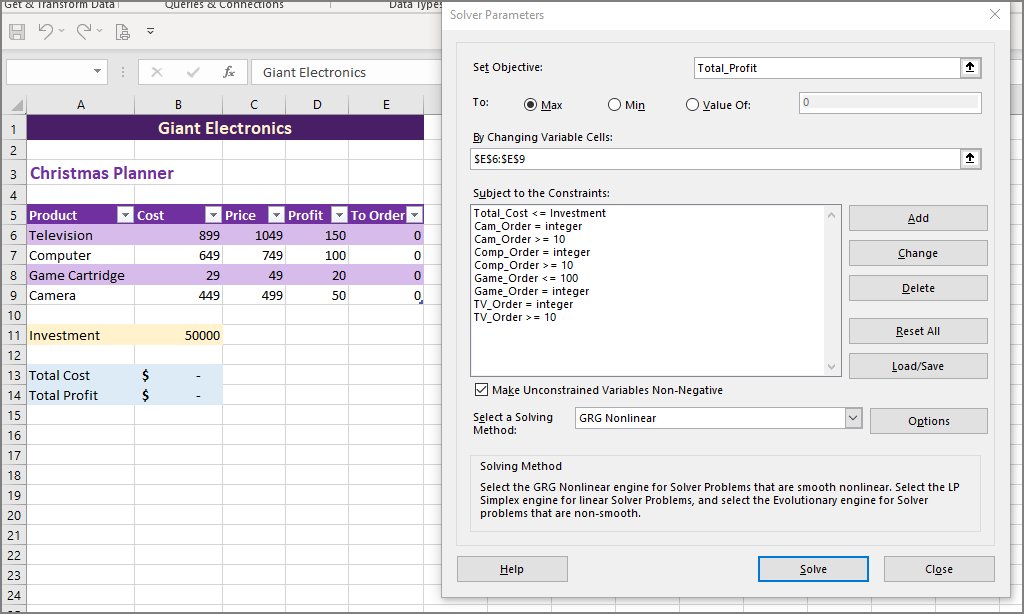
\includegraphics[width=\maxwidth{.95\linewidth}]{gfx/ch08_fig44}
		\caption{Setting Up The Two-Variable Data Table}
		\label{08:fig44}
	\end{figure}

	\item Click \fmtButton{OK}.
\end{enumerate}

The data table displays the payment due for each combination of interest rate and loan term. Borrowers could then use this information to negotiate a rate and term that fits their budget. \textit{Note}: the payments are negative since they represent money leaving the borrower's bank account.

\begin{figure}[H]
	\centering
	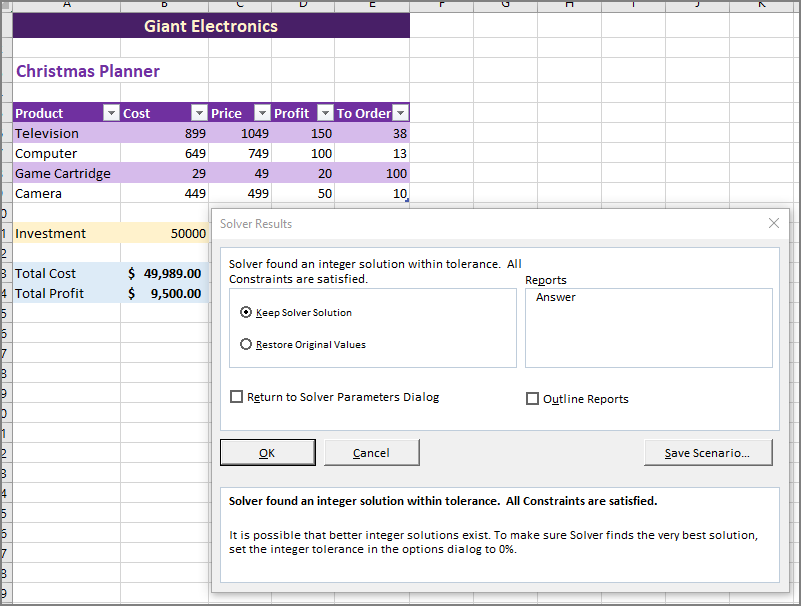
\includegraphics[width=\maxwidth{.95\linewidth}]{gfx/ch08_fig45}
	\caption{Completed Two-Variable Data Table}
	\label{08:fig45}
\end{figure}

\begin{enumerate}[resume]
	\item Save and close the \fmtWorksheet{CH8-Data Table} workbook.
\end{enumerate}

\subsection{Scenarios}

Users may have data in a worksheet and want to change some of the variables to see the effect. For example, a business owner may want to consider ``best case'' and ``worst case'' values and then compare the results. This type of analysis is called a scenario in Excel.

\begin{enumerate}
	\item Open workbook \fmtWorksheet{CH8-Scenario}.
	\item Save the workbook as \fmtWorksheet{CH8-Williams Budget}.
\end{enumerate}

This workbook is a simple household budget for the Williams family. There are two working adults, Morgan and Phoenix. They are planning for several potential changes in their budget, including taking a ``once-in-a-lifetime'' vacation, starting college classes, and purchasing a new home. To help them decide on their best course of action, they are going to develop scenarios.

\begin{enumerate}[resume]
	\item Click \fmtButton{Data $ \Rightarrow $ Forecast $ \Rightarrow $ What-If Analysis $ \Rightarrow $ Scenario Manager}.
	\item Click \fmtButton{Add} in the \textit{Scenario Manager} box.
\end{enumerate}

\begin{figure}[H]
	\centering
	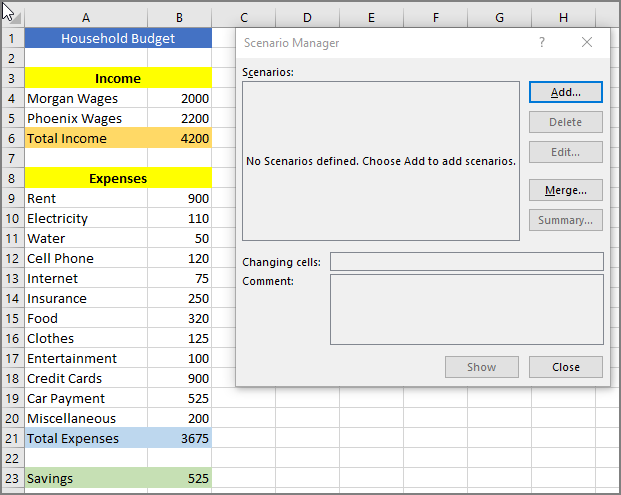
\includegraphics[width=\maxwidth{.95\linewidth}]{gfx/ch08_fig50}
	\caption{The Scenario Manager Dialog}
	\label{08:fig50}
\end{figure}

\begin{enumerate}[resume]	
	
	\item Enter these values in the \textit{Add Scenario} box.
	
	\begin{itemize}
		\item \textbf{Scenario name}: \fmtTyping{Current}. The first scenario will be the current budget and will work as a baseline for the other scenarios.
		\item \textbf{Changing Cells}: \fmtTyping{\$B\$4,\$B\$5,\$B\$9:\$B\$20}. These are the cells that the user can change for each scenario.
		\item \textbf{Comment}: \fmtTyping{Baseline Budget}. This is a brief description of the purpose for this scenario.
		\item \textbf{Prevent Changes}: Checked. This prevents the user from making changes to the Changing Cells other than with the scenario manager.
		\item \textbf{Hide}: Unchecked. This hides all of the changing cells.
	\end{itemize}

\end{enumerate}

\begin{figure}[H]
	\centering
	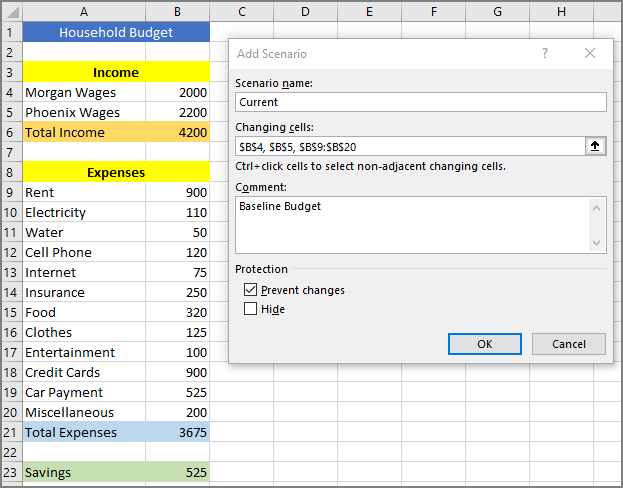
\includegraphics[width=\maxwidth{.95\linewidth}]{gfx/ch08_fig51}
	\caption{Adding A New Scenario}
	\label{08:fig51}
\end{figure}

\begin{enumerate}[resume]

	\item Click \fmtButton{OK}.
	\item The \textit{Scenario Values} box will pop up. This is where the user can insert various values for the changeable cells. For this first scenario, none of the values will be changed, so click \fmtButton{OK}.
	
\end{enumerate}

\begin{figure}[H]
	\centering
	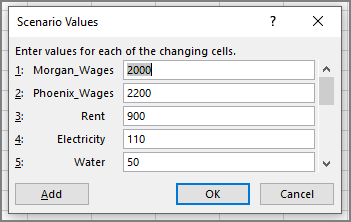
\includegraphics[width=\maxwidth{.75\linewidth}]{gfx/ch08_fig52}
	\caption{Changing Scenario Values}
	\label{08:fig52}
\end{figure}

\begin{enumerate}[resume]	
	
	\item The \textit{Scenario Manager} will pop up. It now indicates that there is one scenario named \textit{Current}. This scenario can be deleted or edited if desired, but click \fmtButton{Add} to create a new scenario.
	
\end{enumerate}

\begin{figure}[H]
	\centering
	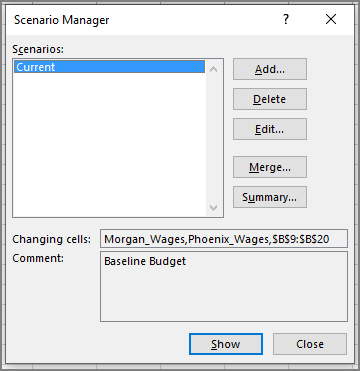
\includegraphics[width=\maxwidth{.65\linewidth}]{gfx/ch08_fig53}
	\caption{Scenario Manager With One Scenario}
	\label{08:fig53}
\end{figure}

\begin{enumerate}[resume]	
	
	\item Enter \fmtTyping{Vacation} for the scenario name, accept the default changing cells, and enter \fmtTyping{Budget for our vacation} as a comment. Leave \textit{Prevent Changes} checked and \textit{Hide} unchecked.
	\item Click \fmtButton{OK}.
	
\end{enumerate}

\begin{figure}[H]
	\centering
	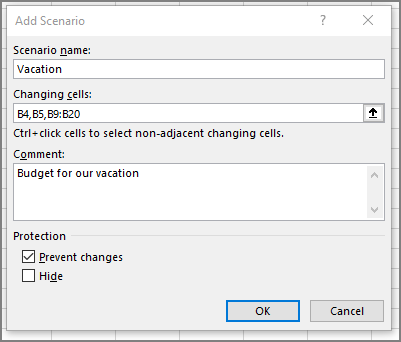
\includegraphics[width=\maxwidth{.75\linewidth}]{gfx/ch08_fig54}
	\caption{The Vacation Scenario}
	\label{08:fig54}
\end{figure}

\begin{enumerate}[resume]	
	
	\item Morgan and Phoenix believe that they need to increase their monthly savings significantly for their vacation. They decide to cut their food budget to $ 250 $, clothes to $ 50 $, entertainment to $ 50 $, and miscellaneous to $ 50 $. Enter those amounts in the \textit{Scenario Values} box.
	
\end{enumerate}

\begin{figure}[H]
	\centering
	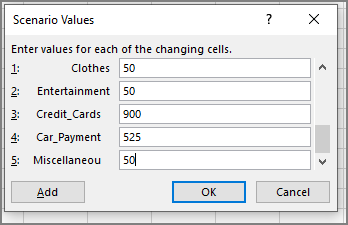
\includegraphics[width=\maxwidth{.65\linewidth}]{gfx/ch08_fig55}
	\caption{Vacation Scenario Values}
	\label{08:fig55}
\end{figure}

\begin{enumerate}[resume]	
	
	\item Click \fmtButton{OK}.
	\item To see the result of the Vacation budget, select \textit{Vacation} and click \fmtButton{Show} on the \textit{Scenario Manager} box.
	
\end{enumerate}

\begin{figure}[H]
	\centering
	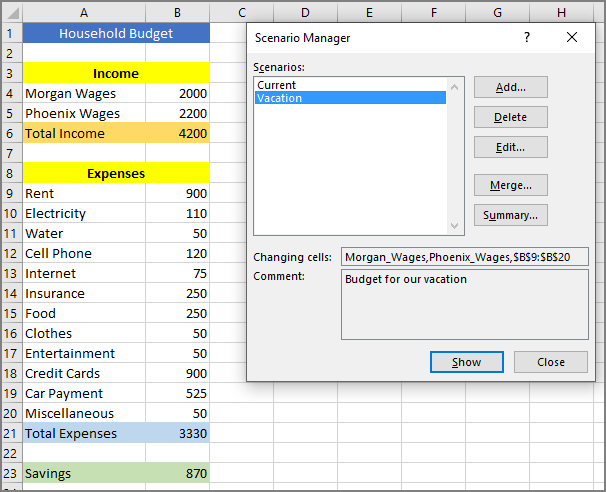
\includegraphics[width=\maxwidth{.95\linewidth}]{gfx/ch08_fig56}
	\caption{Vacation Scenario Results}
	\label{08:fig56}
\end{figure}

\begin{enumerate}[resume]	
	
	\item Morgan and Phoenix can now jump between the \textit{Current} and \textit{Vacation} budgets by selecting them in the \textit{Scenario Manager} box and clicking the \fmtButton{Show} button.
	\item To reset the budget back to its baseline, select \textit{Current} and click \fmtButton{Show} in the \textit{Scenario Manager} box.
	\item Next, they want to consider a budget for if one of them starts college. For that, they believe that they will have to find a smaller apartment near the campus and cut their other expenses significantly.
	\item Click \fmtButton{Add} in the \textit{Scenario Manager}.
	\item Name the new scenario \fmtTyping{College} and enter \fmtTyping{Starting college classes} as a comment. Accept all other default values for this scenario and click \fmtButton{OK}.
	\item In the \textit{Scenario Values} box, enter $ 700 $ for rent, $ 100 $ for electricity, $ 200 $ for insurance, $ 175 $ for food, $ 50 $ for clothes, $ 50 $ for entertainment, and $ 50 $ for miscellaneous, then click \fmtButton{OK}.
	\item To reset the budget back to its baseline, select \textit{Current} and click \fmtButton{Show} in the \textit{Scenario Manager} box.
	\item Finally, Morgan and Phoenix want to consider purchasing a new house. Click \fmtButton{Add} in the \textit{Scenario Manager} box to create a new scenario.
	\item Name the new scenario \fmtTyping{House} and enter \fmtTyping{Possible new house} as a comment. Accept all other default values for this scenario.
	\item Even though they will not have rent, they will have a mortgage payment. For this worksheet, enter 1250 as rent to cover the cost of a mortgage payment. Enter 150 for electricty, 75 for water, 350 for insurance, 250 for food, 75 for clothes, 50 for entertainment, and 100 for miscellaneous.
	\item At this point, there are four scenarios and each can be viewed by clicking its name and \fmtButton{Show} in the \textit{Scenario Manager} box. 
	
\end{enumerate}

\begin{figure}[H]
	\centering
	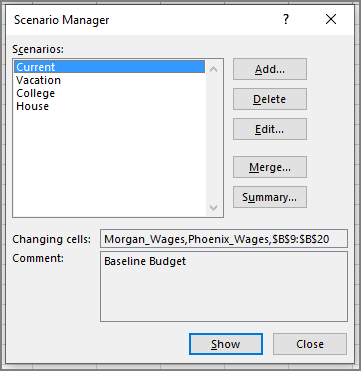
\includegraphics[width=\maxwidth{.75\linewidth}]{gfx/ch08_fig57}
	\caption{The Completed Scenario Manager}
	\label{08:fig57}
\end{figure}

\begin{enumerate}[resume]	
	
	\item It is possible to see a summary of all four scenarios in a single report. Click \fmtButton{Summary} in the \textit{Scenario Manager} box.
	\item Excel offers to create a summary worksheet or a pivot table. For this exercise, select the \fmtButton{Scenario summary} radio button, which will create a report.
	
\end{enumerate}

\begin{figure}[H]
	\centering
	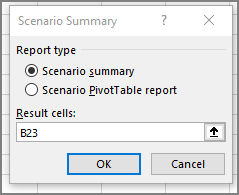
\includegraphics[width=\maxwidth{.55\linewidth}]{gfx/ch08_fig58}
	\caption{Scenario Summary Options}
	\label{08:fig58}
\end{figure}

\begin{enumerate}[resume]	
	
	\item The result cell, \fmtLoc{B23}, is the \textit{Savings} cell and this is the best option for reporting the results of each scenario.
	\item Click \fmtButton{OK}.
	\item Excel produces a nice report that shows the values that were changed for each scenario and the result on their savings. 
\end{enumerate}

\begin{figure}[H]
	\centering
	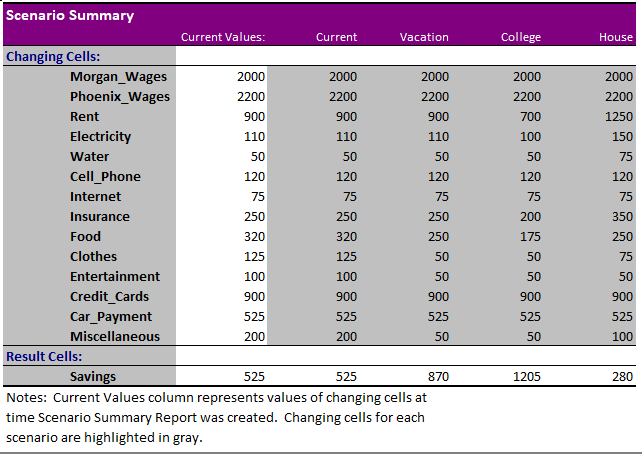
\includegraphics[width=\maxwidth{.95\linewidth}]{gfx/ch08_fig59}
	\caption{Scenario Summary Report}
	\label{08:fig59}
\end{figure}

\begin{enumerate}[resume]
	\item Save and close the \fmtWorksheet{CH8-Williams Budget} workbook.
\end{enumerate}

\subsection{Goal Seeking}

Sometimes it is desirable to calculate a specific output for a formula by changing one of the input variables and this process is called ``Goal Seeking'' in Excel. As a demonstration of Goal Seeking, imagine that a mortgage of $ \$100000 $ is being negotiated and the buyer wants to keep payments under $ \$900 $ per month. If the mortgage will run $ 180 $ months ($ 15 $ years), what interest rate will lead to the maximum monthly payment possible under $ \$900 $?

\begin{enumerate}
	\item Open a new blank workbook.
	\item Rename \fmtWorksheet{Sheet1} to \fmtTyping{Optimum Rate}.
	\item Save the workbook as \fmtWorksheet{CH8-Goal Seek}.
	\item Enter these labels in the first column.

	\begin{itemize}
		\item In cell \fmtLoc{A1} enter \fmtTyping{Loan Amount}.
		\item In cell \fmtLoc{A2} enter \fmtTyping{Term in Months}.
		\item In cell \fmtLoc{A3} enter \fmtTyping{Interest Rate}.
		\item In cell \fmtLoc{A4} enter \fmtTyping{Payment}.
	\end{itemize}

	\item Adjust the width of \fmtLoc{Column A} so the labels fit in the column.
	\item Enter the following known values.

	\begin{itemize}
		\item In cell \fmtLoc{B1} enter \fmtTyping{$ 100000 $}. This is the amount being borrowed.
		\item In cell \fmtLoc{B2} enter \fmtTyping{$ 180 $}. This is the number of months to pay off the loan. 
		\item In cell \fmtLoc{B4} enter \fmtTyping{=PMT(B3/12,B2,B1)} to calculate the payment. 
	\end{itemize}

	\item Because there is no value in cell \textit{B3}, Excel assumes a $ 0 $\% interest rate and returns a payment of \$$ 555.56 $. That value can be ignored for now.
\end{enumerate}

Use \textit{Goal Seek} to determine the optimum interest rate for the payment desired.

\begin{enumerate}
	\item Click \fmtButton{Data $ \Rightarrow $ Forecast $ \Rightarrow $ What-If Analysis $ \Rightarrow $ Goal Seek}.
	\item In the \textit{Set cell} box, enter the reference for the cell that contains the formula to be resolved. In the example, this formula is in cell \fmtLoc{B4}.
	\item In the \textit{To value} box, enter the desired result \fmtTyping{-900}. \textit{Note} this number is negative because it represents money being paid out of a checking account.
	\item In the \textit{By changing cell} box, enter the reference for the cell that contains the value to adjust, or \fmtLoc{B3} in this example. \textit{Note}: The cell that \textit{Goal Seek} changes must be referenced by the formula in the cell specified in the \textit{Set cell} box.
	
\end{enumerate}

\begin{figure}[H]
	\centering
	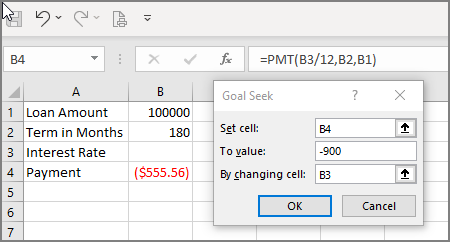
\includegraphics[width=\maxwidth{.95\linewidth}]{gfx/ch08_fig60}
	\caption{Setting Up Goal Seeking}
	\label{08:fig60}
\end{figure}

\begin{enumerate}[resume]	
	\item Click \fmtButton{OK}.
\end{enumerate}

Excel calculates an interest rate of $ 0.07021 $ ($ 7\% $) to yield a monthly payment of $ \$900 $. 

\begin{enumerate}[resume]
	\item To save the calculated amounts in the worksheet, click \textit{OK} but to cancel this process and return to the original worksheet values, click \textit{Cancel}. For this exercise, click \fmtButton{OK}.
	\item Save and close the \fmtWorksheet{CH8-Goal Seek} workbook.
\end{enumerate}

\begin{figure}[H]
	\centering
	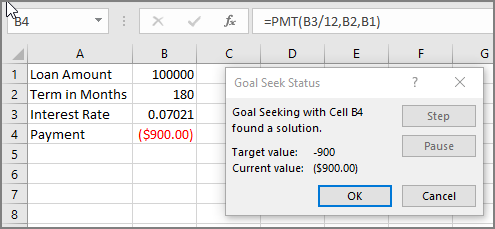
\includegraphics[width=\maxwidth{.95\linewidth}]{gfx/ch08_fig61}
	\caption{Results of Goal Seeking}
	\label{08:fig61}
\end{figure}

\subsection{Solver}

The Excel Solver is used to find an optimum solution for complex business problems. As an example, Solver would evaluate multiple parameters to find the best mix of products for a company to manufacture. For this exercise, the \textit{PeopleMover Transportation} company wants to create a spreadsheet that will help their planners determine the best mix of motor coaches for a contract.

\begin{enumerate}
	\item Open workbook \fmtWorksheet{CH8-Solver}.
	\item Save the workbook as \fmtWorksheet{CH8-PeopleMover}.
\end{enumerate}

This workbook has only one worksheet, \textit{Planner}. The worksheet has some information already filled in. The company has four different coaches: \textit{Deluxe}, \textit{Large}, \textit{Mid-Size}, and \textit{Mini}. For each type of coach, the passenger capacity is listed. Also, the cost of operating the coach per mile is specified. Finally, the number that the company has on hand is listed. For example, a \textit{Deluxe} coach can carry $ 56 $ passengers at a cost of \$$ 2.80 $ per mile to operate. The company has two \textit{Deluxe} coaches on hand.

Cells \textit{A14:B15} on the worksheet is where information about a trip is entered. For example, the worksheet is set up for a trip of $ 300 $ miles that a group of $ 350 $ people want to take.

The goal is to have Excel calculate the optimum mix of coaches to get a total capacity (cell \textit{B11}) greater than the number of riders (\textit{B15}) at a minimum cost (cell \textit{B12}). This is a perfect job for \textit{Solver}.

\textit{Solver} is part of Excel, but it is considered an Add-in and must be activated before it can be used. Note: this process only needs to be done one time, so if \textit{Solver} is already activated, this part of the exercise can be skipped.

\begin{enumerate}[resume]
	\item Click \fmtButton{File} to open the backstage view.
	\item In the backstage view, click \fmtButton{Options} at the bottom of the left-hand menu.
	
\end{enumerate}

\begin{figure}[H]
\centering
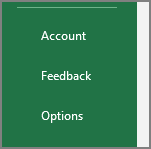
\includegraphics[width=\maxwidth{.40\linewidth}]{gfx/ch08_fig70}
\caption{The Options Button in the Backstage View}
\label{08:fig70}
\end{figure}

\begin{enumerate}[resume]	
	
	\item Click \fmtButton{Add-ins} in the left-hand menu of the \textit{Excel Options} pop-up box.
	\item Select \textit{Excel Add-ins} in the drop-down menu at the bottom of the \textit{Add-ins} tab.
	\item Click \fmtButton{Go}.
	
\end{enumerate}

\begin{figure}[H]
\centering
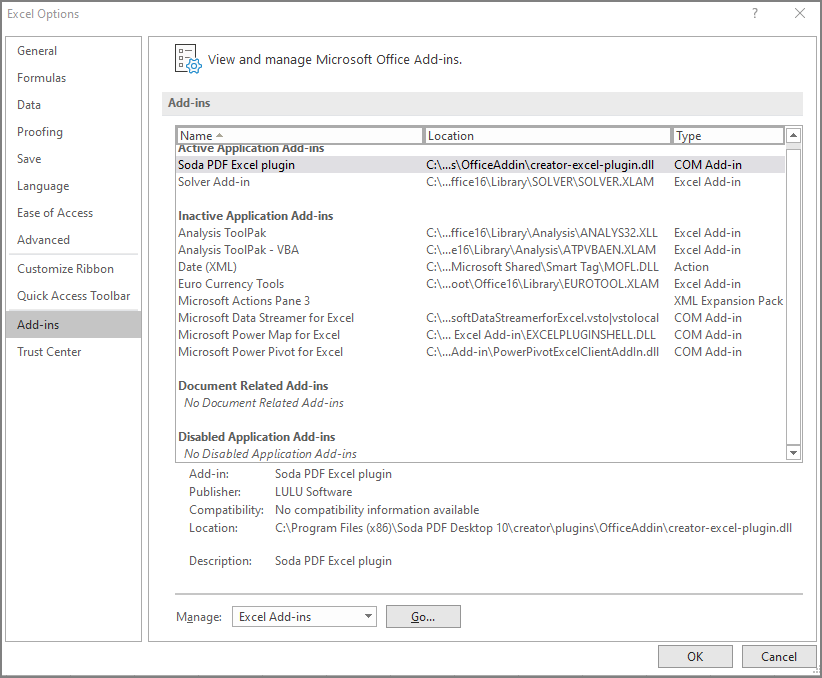
\includegraphics[width=\maxwidth{.95\linewidth}]{gfx/ch08_fig71}
\caption{The Add-ins Manager}
\label{08:fig71}
\end{figure}

\begin{enumerate}[resume]	
	
	\item Click the checkbox beside \textit{Solver Add-in} in the \textit{Add-ins} pop-up box.
	
\end{enumerate}

\begin{figure}[H]
	\centering
	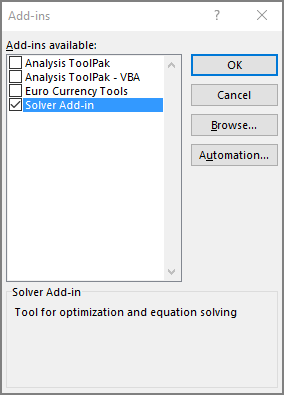
\includegraphics[width=\maxwidth{.65\linewidth}]{gfx/ch08_fig72}
	\caption{Activating The Solver Add-In}
	\label{08:fig72}
\end{figure}

\begin{enumerate}[resume]	
	\item Click \fmtButton{OK}.
\end{enumerate}

Notice that there is a new \textit{Solver} button at \textit{Data $ \Rightarrow $ Analyze}.

\begin{enumerate}[resume]
	\item To set up the solver, click \fmtButton{Data $ \Rightarrow $ Analyze $ \Rightarrow $ Solver}.
	\item In the \textit{Set Objective} box, click the selector button and then click cell \fmtLoc{B12} to select it. This sets the \textit{Solver} to solve for the total cost of the coaches. (Note: since cell \fmtLoc{B12} has a name, the \textit{Solver}  may display the name \textit{Ttl\_Cost} instead of \fmtLoc{B12}.)
	\item For \textit{To}, Select the \fmtButton{Min} radio button. This sets the \textit{Solver} to look for the minimum cost for the mix of coaches it recommends.
	\item For \textit{By Changing Variable Cells} enter \fmtTyping{\$E\$6:\$E\$9}. This tells Excel to change the number of coaches allotted in order to minimize the cost for the number of passengers to carry.
	\item Click \fmtButton{Add} beside the \textit{Subject to the Constraints} box to add the constraints for the \textit{Solver}.
	\item Specify that cell \fmtLoc{E6} must be $ <= $ cell \fmtLoc{D6}. That means that the number of \textit{Deluxe} coaches allotted for the trip must be less than or equal to the number on hand.
	\item Click \fmtButton{Add} to add another constraint.
	\item Specify that cell \fmtLoc{E6} must be an \fmtButton{int} since it is not possible to allot a partial coach.
	\item Click \fmtButton{OK} to return to the \textit{Solver Parameters} dialog box. 
	\item There are now two constraints, but the cell names are used rather than the location identifiers. The first constraint requires the number of coaches allotted be less than the number on hand and the second requires only complete coaches be allotted.
	\item Add constraints for Large, Mid-Size, and Mini coaches that are similar to those for the Deluxe coach.
	\item Add a constraint that \fmtLoc{B11} must be $ >= $ \fmtLoc{B15} since all riders need to have a seat on a coach.
	\item Check the box for ``Make Unconstrained Variables Non-Negative'' since it is not possible to have a negative number of coaches or riders.
	 \item For \textit{Select a Solving Method}, the default is \fmtButton{GRG Nonlinear}. This is normally a good option to use.
	 
\end{enumerate}

\begin{figure}[H]
	\centering
	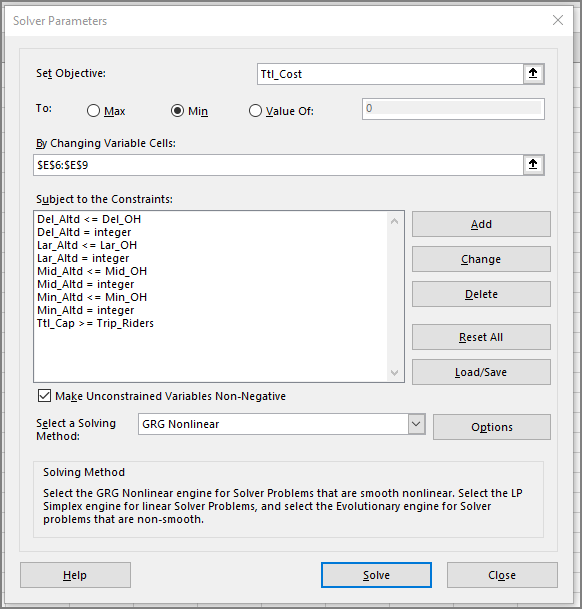
\includegraphics[width=\maxwidth{.95\linewidth}]{gfx/ch08_fig73}
	\caption{The Solver Parameters}
	\label{08:fig73}
\end{figure}

\begin{enumerate}[resume]	 
	 \item Click \fmtButton{Solve}.
\end{enumerate}

After a few seconds, the Solver will calculate the mix of coaches that yields the least cost. Notice that the \textit{Solver} changed the \textit{Allotted} values for each of the coaches along with the \textit{Total Capacity} and \textit{Total Cost} to match the optimal solution. Also, notice that the total coach capacity is $ 354 $ for the solution while there are only $ 350 $ riders, so there will be four empty seats on the coaches. This solution will cost \textit{PeopleMover Transportation} \$$ 4,575.00 $ so they would have to price tickets appropriately.

\begin{figure}[H]
	\centering
	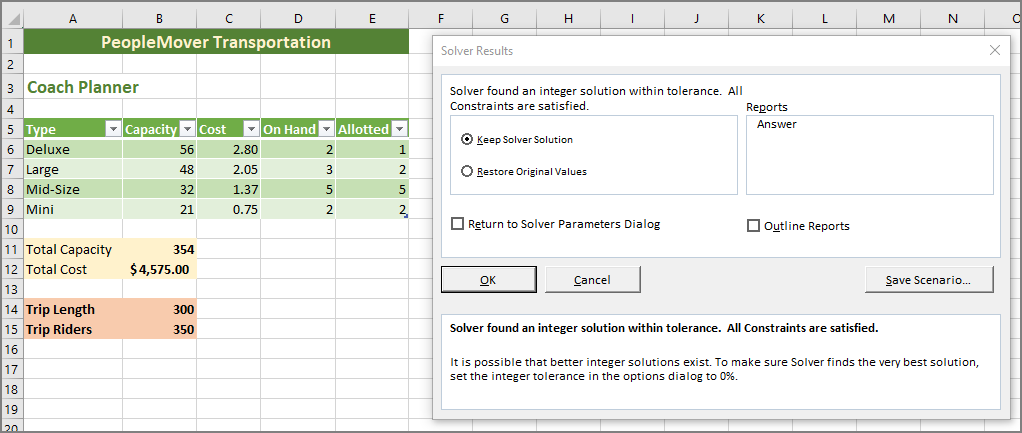
\includegraphics[width=\maxwidth{.95\linewidth}]{gfx/ch08_fig74}
	\caption{Solver Results}
	\label{08:fig74}
\end{figure}

\begin{enumerate}[resume]
	\item Click \fmtButton{Keep Solver Solution} and \fmtButton{OK} to save this solution. (To return to the original values without saving, click \textit{Restore Original Values} and \textit{OK}. Finally, this solution can be saved as a scenario so it can be compared with other solutions.)
	\item Save and close \fmtWorksheet{CH8-PeopleMover}.
\end{enumerate}

\begin{center}
	\begin{tkwbox}{Key Take-Aways}
		\textbf{What-If Analysis}
		\\
		\begin{itemize}
			\setlength{\itemsep}{0pt}
			\setlength{\parskip}{0pt}
			\setlength{\parsep}{0pt}
			
			\item Data tables are built by processing numeric inputs using Excel functions and formulas.
			\item Scenarios create various sets of inputs to compare the resulting output.
			\item Goal seeking finds an optimum input to achieve a specific goal.
			\item The Solver finds optimal solutions to complex business problems.
			
		\end{itemize}
	\end{tkwbox}
\end{center}

\section{Chapter Practice}

\subsubsection{Electoral College Votes}

The United States Electoral College is a unique institution that is responsible for electing the President. In theory, people vote for electors in November who then meet in December to vote for the President. This exercise draws a \textit{$ 3 $D Map} of the Electoral College presidential votes since $ 1912 $.

\begin{enumerate}
	\item Open \fmtWorksheet{PR8-Data}. This workbook contains the results of the electoral college vote\footnote{The electoral college data was found at the United States National Archives, \url{https://www.archives.gov/electoral-college}} for all US Presidential elections from $ 1912 $ until $ 2016 $. Notes: In the $ 1912 $ election, Theodore Roosevelt ran under the ``Progressive'' party but his votes are listed as ``Republican'' in this document since there was no Republican candidate that year. Alaska and Hawaii first sent delegates to the electoral college in $ 1960 $ and Washington DC in $ 1964 $.
	\item Save the workbook as \fmtWorksheet{PR8-Elections}.
	\item Click in \fmtLoc{A1} to activate that cell.
	\item Click \fmtButton{Insert $ \Rightarrow $ Tours $ \Rightarrow $ 3D Map}.
	\item If Excel did not automatically place the \textit{State} data field in the \fmtButton{Location} setting, then click and drag \textit{State} in the \textit{Electoral\_College Field List} to the \fmtButton{Location} setting. 
	\item Click the down arrow to the right of \textit{State} in the \textit{Location} setting and select \fmtButton{State/Province} in the drop down list.
	\item Click the pencil icon beside \textit{Layer 1} and change the name of this layer to \fmtTyping{Votes}.
	\item Click and drag \textit{Votes} in the \textit{Electoral\_College Field List} to the \fmtButton{Height} setting.
	\item Click and drag \textit{Year} in the \textit{Electoral\_College Field List} to the \fmtButton{Time} setting.
	\item Click the down arrow to the right of \textit{Year} in the \textit{Time} setting and select \fmtButton{Year} in the drop down list.
	\item Click and drag \textit{Party} in the \textit{Electoral\_College Field List} to the \fmtButton{Category} setting.
	\item Change the visualization type to \fmtButton{Bubble}.
	\item Click the down arrow to the right of \textit{Votes} in the \textit{Size} setting and select \fmtButton{No Aggregation} in the drop down list.
	\item Click \fmtButton{Flat Map} and then adjust the map to fit on the screen. Remember that Alaska and Hawaii need to be visible on the map. Also, experiment with the four arrow and plus/minus buttons to adjust the display.
	\item Under Layer Options, change the color for \textit{Republican} to red and \textit{Other} to green.
	\item Play the tour to see what it looks like.
	\item Click \textit{Tour 1} at the top of the \textit{Tour Editor}. Enter \fmtTyping{Election} as the name of the tour. 
	\item The displayed date shows the day, month, and year, but election results only change every four years. To make the date display more appropriate, right-click it and select \fmtButton{Edit}. In the edit box, choose the \textit{Time Format} that only shows the year without the month and day. Change the background color of the date display to white. Click \fmtButton{Accept} to lock in these changes. 
	\item Once the date is adjusted, resize and position it so it does not cover any of the states. 
	\item Add a text box with the title of \fmtTyping{Elections} and this description: \fmtTyping{Results of the Electoral College votes for 1912-2016}. Set the background color of the text box to white. Once the box is created, resize and position it so it does not cover any of the states.
	\item Resize and position the legend box so it does not cover any of the states.
	\item Click the \fmtButton{Scene Options} button on the ribbon and change the name of the scene to \fmtTyping{Elections}.
	\item Click \fmtButton{Map Labels} to turn on the labels.
	\item Click \fmtButton{Tour Editor}, \fmtButton{Layer Pane}, and \fmtButton{Field List} to turn off those dialog boxes. These can always be turned back on if desired.
	\item Play the tour to view the final version.
	
	\begin{figure}[H]
		\centering
		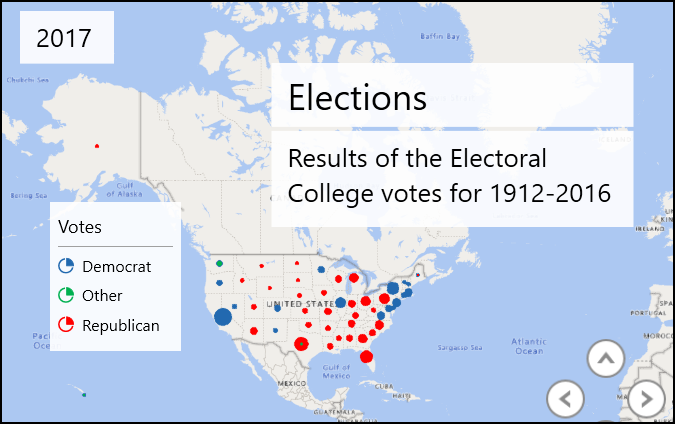
\includegraphics[width=\maxwidth{.95\linewidth}]{gfx/ch08_fig80}
		\caption{Electoral College Map}
		\label{08:fig80}
	\end{figure}
	
	\item Click \fmtButton{Create Video} to create a video version of the tour.
	\item In the \textit{Create Video} dialog box, select \fmtButton{Quick Export \& Mobile}, then click \fmtButton{Create}. Save the video in the same folder as \fmtWorksheet{PR8-Elections}. Note: The video is being created at the lowest possible resolution so the file is small to make it easier to submit it to the instructor; to create a video designed to be presented to clients, it should be created at a higher resolution.
	\item To save the map, click \fmtButton{File $ \Rightarrow $ Close}. The map is saved as part of the workbook and will be available the next time the workbook is opened.
	\item Save and close the \fmtWorksheet{PR8-Elections} workbook.
	\item Submit the \fmtWorksheet{PR8-Elections} workbook and video to the instructor.
\end{enumerate}


\section{Scored Assessment}

\subsection{Product Mix}

The \textit{Giant Electronics} company is a local small business that sells discounted electronic devices, like televisions and computers. The owners, Addison and Kelsey, are planning for their annual spring promotion and want to create a good mix of sale items.

\begin{enumerate}
	\item Open workbook \fmtWorksheet{SC8-Data}.
	\item Save the workbook as \fmtWorksheet{SC8-Product Mix}.
\end{enumerate}

This workbook has only one worksheet, \textit{Planner}. The worksheet already has some information filled in. Addison and Kelsey are planning to promote four items, a television, a computer, various game cartridges, and a camera. The worksheet shows the cost for each item; for example, each television set costs them \$$ 899 $. The price they intend to sell each item is also noted. For example, televisions will sell for \$$ 1049 $. The profit for each item is calculated by subtracting the cost from the price. Finally, the \textit{To Order} column lists how many of each item they should order for their sale.

In cell \textit{B11}, under the Planner table, Addison and Kelsey indicate how much they want to invest in the sale. The worksheet initially indicates a \$$ 50,000 $ investment.

Cell \textit{B13} has a formula that calculates the total cost of whatever they decide to order and \textit{B14} has a formula that calculates the total profit for those items.

\begin{enumerate}
	\item Click \fmtButton{Data $ \Rightarrow $ Analyze $ \Rightarrow $ Solver}.
	\item In the \textit{Set Objective} box, click the selector button and then click cell \fmtLoc{B14} to select it. This sets the Solver to solve for the total profit of the sale items. (Note: since cell \fmtLoc{B14} has a name, the Solver may display 	the name \textit{Total\_Profit} instead of \fmtLoc{\$B\$14}.)
	\item For \textit{To}, Select the \fmtButton{Max} radio button. This sets the Solver to look for the maximum profit for the mix of products it recommends.
	\item The constraints are already defined. These will be changed later, but the initial configuration requires the total cost to be less than the investment. The configuration also requires all orders to be integers (it is not possible to order a fraction of a television) and there are some constraints on the number of items that can be ordered.
	\item Make sure the \textit{GRG Nonlinear} is the solving method.
\end{enumerate}

\begin{figure}[H]
	\centering
	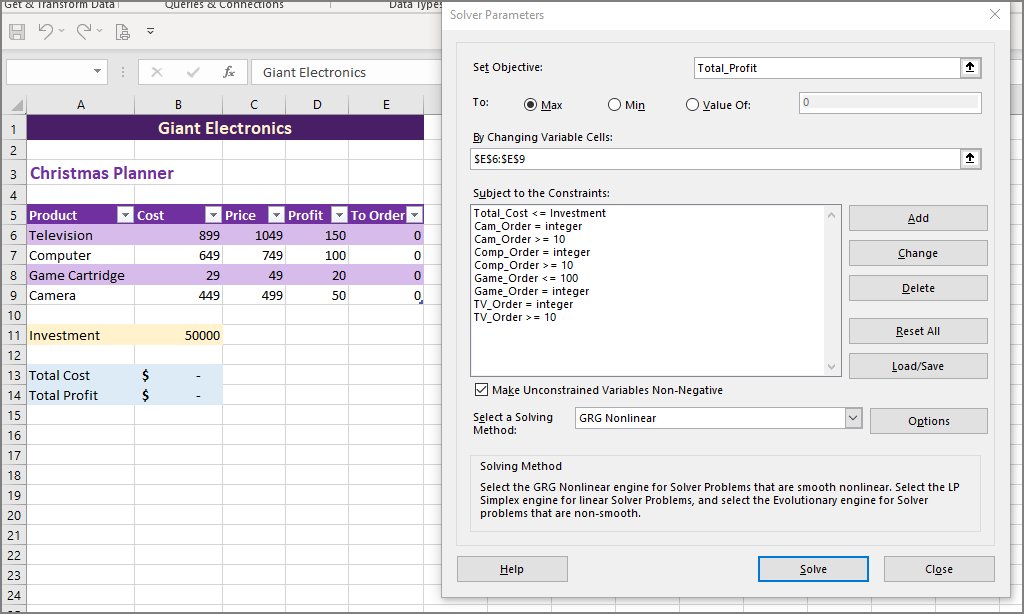
\includegraphics[width=\maxwidth{.95\linewidth}]{gfx/ch08_fig81}
	\caption{Solver Initial Setup}
	\label{08:fig81}
\end{figure}

\begin{enumerate}[resume]
	\item Click \fmtButton{Solve}.
\end{enumerate}

\begin{figure}[H]
	\centering
	\includegraphics[width=\maxwidth{.95\linewidth}]{gfx/ch08_fig82}
	\caption{Solver Initial Solution}
	\label{08:fig82}
\end{figure}

Solver determined that the optimum mix of products was $ 38 $ televisions, $ 13 $ computers, $ 100 $ Game cartridges, and $ 10 $ cameras. This will cost Addison and Kelsey \$$ 49,989 $, just under their \$$ 50,000 $ limit and will net them a profit of \$$ 9,500 $. 

\begin{enumerate}[resume]
	\item Click \fmtButton{Save Scenario}.
	\item Name the scenario \fmtTyping{Initial Attempt} and click \fmtButton{OK}.
	\item Click \textit{Restore Original Values} in the Results dialog box to return the Planner table to its original state.
	\item Click \textit{Answer} in the Reports dialog box. This makes Excel generate a report named \textit{Answer Report 1}.
	\item Click \fmtButton{OK}.
	\item Excel creates a report on a new worksheet named \fmtWorksheet{Answer Report 1}. This makes it easy to come back to this solution later.
	\item Click \fmtButton{Data $ \Rightarrow $ Forecast $ \Rightarrow $ What-If $ \Rightarrow $ Scenario Manager}.	Notice that Excel placed that first scenario, \textit{Initial Attempt}, in the scenario manager for later reference.
	\item Click \fmtButton{Close} to close the scenario manager.
\end{enumerate}

Addison and Kelsey decide that they want to sell more than $ 10 $ cameras and they think that $ 100 $ game cartridges are too many. 

\begin{enumerate}
	\item Click \fmtButton{Data $ \Rightarrow $ Analyze $ \Rightarrow $ Solver}.
	\item Click \textit{Cam\_Order $ >=$ $ 10 $} to select it and then click \fmtButton{Change}.
	\item Change the constraint to $ 20 $ and click \fmtButton{OK}.
	\item Click \textit{Game\_Order $ <=$ $ 100 $} to select it and then click \fmtButton{Change}.
	\item Change the constraint to $ 50 $ and click \fmtButton{OK}.
	\item Click \fmtButton{Solve}.
	\item Notice that Excel has now adjusted the order column so only $ 50 $ game cartridges and $ 20 $ cameras will be ordered. Also notice that the profit has dropped to \$$ 8,500 $. 
	\item Click \fmtButton{Save Scenario}, name it \fmtTyping{20 Cameras}, and click \fmtButton{OK}.
	\item Click \textit{Answer} in the Reports dialog box. This makes Excel generate a report named \textit{Answer Report 2}.
	\item Select \textit{Restore Original Values} and click \fmtButton{OK}.
\end{enumerate}

Addison and Kelsey would like to boost their profit a bit so they decide to adjust the selling price for two items. They think the television could sell for \$$ 1199 $ and the computer for \$$ 999 $. 

\begin{enumerate}
	\item Click \fmtLoc{C6} to activate that cell and enter $ 1199 $ for the new television selling price.
	\item Click \fmtLoc{C7} to activate that cell and enter $ 999 $ for the new computer selling price.
	\item Click \fmtButton{Data $ \Rightarrow $ Analyze $ \Rightarrow $ Solver}.
	\item Click \fmtButton{Solve} on the \textit{Solver Parameters} dialog box.
	\item Click \fmtButton{Save Scenario}, name it \fmtTyping{Expensive Televisions}, and click \fmtButton{OK}.
	\item Click \textit{Answer} in the Reports dialog box. This makes Excel generate a report named \textit{Answer Report 3}.
	\item Select \textit{Restore Original Values} and click \fmtButton{OK}.
\end{enumerate}

Addison and Kelsey could continue adjusting the sale prices and the maximum number of each item to order to come to what they believe is the optimum mix of products for their spring sale.

Take a look at \textit{Answer Report 1}, \textit{Answer Report 2}, and \textit{Answer Report 3} to compare the results of each scenario. It would be easier to see all three scenarios in a single report.

\begin{enumerate}[resume]
	\item Click \fmtButton{Data $ \Rightarrow $ Forecast $ \Rightarrow $ What-If Analysis $ \Rightarrow $ Scenario Manager}.
	\item Notice that all three scenarios are listed. To create a single report containing all scenarios, click \fmtButton{Summary}.
	\item In the Scenario Summary diaglog box, make sure \textit{Scenario Summary} is selected and the result cells are \fmtLoc{B13},\fmtLoc{B14}.
	\item Click \fmtButton{OK}. The report illustrated in Figure \ref{08:fig83} is created.

	\begin{figure}[H]
		\centering
		\includegraphics[width=\maxwidth{.95\linewidth}]{gfx/ch08_fig83}
		\caption{Solver Scenario Summary}
		\label{08:fig83}
	\end{figure}

	\item Save and close the \fmtWorksheet{SC8-Product Mix} workbook.
	\item Submit the \fmtWorksheet{SC8-Product Mix} workbook to the instructor.
\end{enumerate}

\section{Addendum: Filled Map}

\begin{center}
	\begin{infobox}{Information}
		\textbf{Filled Maps}
		\\
		\\
		This section concerns creating a 2-D Filled Map in an Excel workbook. These maps are very useful and easy to create, but are only available for Excel $ 2016 $ installations that include a subscription to Excel $ 365 $.
	\end{infobox}
\end{center}

After Excel $ 2016 $ was released, Microsoft added a new feature, \textit{Filled Maps}. This feature was added to Excel installations that included an Office 365 subscription, but not to stand-alone installations. As a result, some Excel $ 2016 $ installations will have \textit{Filled Maps} available but others will not. This addendum was included with this chapter for students who have access to \textit{Filled Maps}, but it is not considered part of the formal Excel training course.

\begin{enumerate}
	\item Open workbook \fmtWorksheet{CH8-CancerRate}. This workbook contains the rate of cigarette smoking along with cancer rates for various types of cancer that seem to be related to smoking. The data was captured in a study completed in $ 1960 $.
	\item Save the workbook as \fmtWorksheet{CH8-Cancer Map}.
	\item Click cell \fmtLoc{A3:B43} to activate that range of cells.
	\item Click \fmtButton{Insert $ \Rightarrow $ Charts $ \Rightarrow $ Maps $ \Rightarrow $ Filled Map}.
\end{enumerate}

\begin{figure}[H]
	\centering
	\includegraphics[width=\maxwidth{.95\linewidth}]{gfx/ch08_fig90}
	\caption{Creating a Filled Map}
	\label{08:fig90}
\end{figure}

\begin{enumerate}[resume]	
	\item Excel creates a map of the United States with the cigarette use rate indicated by color. Nebraska has the highest rate of cigarette use and states that are gray, like Oregon, did not have data in the input table.
	\item Click the chart title two times to enable editing. Change that title to \fmtTyping{Cigarette Use}.
	\item Click the paint brush tool at the top right corner of the map to change the style and colors for the map. Click \fmtButton{Color} in the popup menu.
	\item Select \fmtButton{Monochromatic Palette 6}, a green palette.
\end{enumerate}

\begin{figure}[H]
	\centering
	\includegraphics[width=\maxwidth{.95\linewidth}]{gfx/ch08_fig91}
	\caption{Completed Map}
	\label{08:fig91}
\end{figure}

\begin{enumerate}[resume]
	\item Save and close the \fmtWorksheet{CH8-Cancer Map} workbook.
\end{enumerate}

In the same way that the cigarette use rate was mapped, any of the types of cancer can be mapped. The limitation is that only one variable, plus the state names, can be mapped at one time. However, if managers had sales data available, this would be a great way to determine, for example, where their best customers live so they can plan some sort of promotion.



